\documentclass{article}

\newcommand{\ts}{\textsuperscript}
\newcommand{\figref}[1]{Fig.~\ref{#1}}
\usepackage{amsmath}
\usepackage{amsthm}
\usepackage{graphicx}
\usepackage{geometry}
\usepackage{subcaption}
\usepackage{bm}
\usepackage{hyperref}
\usepackage[retainorgcmds]{IEEEtrantools}
\usepackage{mathtools}
\usepackage{color}
\usepackage{marginnote}
\usepackage[utf8]{inputenc}


\DeclareMathOperator*{\argmax}{arg\,max}
\DeclareMathOperator*{\argmin}{arg\,min}
\DeclareMathOperator{\st}{s.t.}
\DeclareMathOperator{\epi}{epi}
\DeclareMathOperator{\diag}{diag}
\DeclareMathOperator{\dom}{dom}
\DeclareMathOperator{\tr}{tr}
\DeclareMathOperator*{\minimize}{minimize}
\DeclarePairedDelimiter\floor{\lfloor}{\rfloor}

\newcommand{\iso}{\simeq}
\newcommand{\dd}{\partial}
\newcommand{\real}{\bm R}
\newcommand{\trueRisk}{R_{\mathrm{true}}}

\newcommand{\starsection}{\vspace{1em}\begin{center}$\star\quad\star\quad\star$\end{center}\vspace{1em}}


\newcommand{\hilight}[1]{\colorbox{yellow}{#1}}
\let\oldmarginnote\marginnote
\renewcommand{\marginnote}[1]{\oldmarginnote{\footnotesize\emph{#1}}[0cm]}

\theoremstyle{plain}
\newtheorem{prop}{Proposition}
\newtheorem{thm}{Theorem}

\theoremstyle{definition}
\newtheorem*{deff}{Definition}
\newtheorem*{rem}{Remark}


\geometry{letterpaper}
\IEEEeqnarraydefcolsep{0}{\leftmargini}


\title{Generalization Bounds for Regularized Portfolio Selection with Market Side Information}
\author{
  Erick Delage\\
  Department of Decision Sciences\\
  HEC Montreal\\
  Montreal...\\
  \texttt{erick.delage@hec.ca}\\
  \And
  Thierry Bazier-Matte\\
  HEC Montreal\\
  \texttt{thierry.bazier-matte@hec.ca}\\
}

\begin{document}
\maketitle

\begin{abstract}
%  In recent years,  much pressure has been applied in order to allow portfolio management theory to address was required to evolve in order to  
  Drawing on statistical learning theory, we derive out-of-sample and suboptimal
  guarantees about the investment strategy obtained from a regularized portfolio
  optimization model which attempts to exploit side information about the financial market
  in order to reach an optimal risk-return tradeoff. This side information might include
  for instance recent stock returns, volatility indexes, financial news indicators,
  etc. In particular, we demonstrate that an investment policy that linearly combines this
  side information in a way that is optimal from the perspective of a random sample set is
  guaranteed to perform also relatively well (\ie, within an additive perturbation factor
  of $O(1/\sqrt{n})$) with respect to the unknown distribution that generated this sample
  set. Finally, we evaluate the sensitivity of these results in a high dimensional regime
  where the size of the side information vector is of an order that is comparable to the
  sample size.

  % \Erick{Voici l'ancien abstract: Drawing on statistical learning theory, we propose a
  %   robust portfolio optimization mechanism agnostic to market distribution based on side
  %   information and on market returns. In particular, we exhibit a linear investment
  %   policy based on the risk preferences of an investor and on a sample of the market and
  %   show that out-of-sample and suboptimality guarantees on the quality of the certainty
  %   equivalent of the proposed investment can be provided. In addition, we also consider
  %   the high dimensional case where the number of these side informations is of the order
  %   of the sample size. }
\end{abstract}

\section{Introduction}

\subsection{Exposition du problème et hypothèses}

Ce mémoire vise à établir clairement et rigoureusement comment un investisseur
\textit{averse au risque} disposant \textit{d'information complémentaire} au
\textit{marché} peut utiliser cette information pour accroître son \textit{utilité
  espérée} ou, de façon équivalente, son \textit{rendement équivalent certain}.

\paragraph{Modélisation du marché}

Nous entendrons ici par \textit{marché} n'importe quel type d'actif financier ou
spéculatif dans lequel on peut investir une partie de sa fortune dans l'espoir de la voir
fructifier au cours d'une période de temps arbitraire. Ainsi, tout au long de l'exposé
théorique qui suivra, il peut être pertinent d'avoir en tête les rendements quotidiens
issus des grands indices boursiers (par exemple les 500 plus grandes capitalisations
américaines). Cependant, le traitement qui sera développé pourrait tout aussi bien
s'appliquer à une action cotée en bourse dont on considère les rendements mensuels.\nec
Mathématiquement, l'idée de marché peut ainsi être réduite à celle d'une variable
aléatoire $R(t)$ décrivant l'évolution du rendement de l'actif en question.

Relativement à l'idée de marché, nous ferons également l'hypothèse que l'univers a une
influence sur ces rendements. Il serait par exemple raisonnable de croire que le prix du
pétrole a une influence sur l'évolution du rendement du marché américain. De la même
façon, l'annonce d'un scandale aura a son tour des répercussions sur la valeur du titre de
la compagnie dont il est l'objet. En outre, il a été montré par Fama et French que le
rendement d'une action pouvait s'expliquer comme une combinaison de quelques facteurs
fondamentaux (la taille de l'entreprise, le risque de marché et le ratio cours/valeur). On
peut alors considérer un vecteur d'information $\vec X(t) = (X_1(t), X_2(t), \dots)$ dont
chaque composante représente une information particulière, par exemple l'absence ou la
présence d'un certain type de scandale, un ratio comptable, le prix d'un certain actif
financier\reph. D'un point de vue probabiliste, on dira donc qu'il existe une forme de
dépendance entre $R(t)$ et $\{\vec X(\tau) \mid \tau < t\}$ l'ensemble des évènements antérieurs à
$t$. Le processus joint de ces deux évènements sera désormais défini comme \textit{la
  distribution totale de marché}, ou simplement le marché.


\paragraph{Stationarité}

Bien qu'un tel modèle permette de représenter de façon très générale l'évolution d'un
marché, nous formulerons l'hypothèse supplémentaire selon laquelle le marché est un
processus \textit{stationnaire}. Ceci permet notamment d'évacuer la notion temporelle afin
de ne représenter qu'une distribution de causes (l'information $X$) et d'effet
(l'observation des rendements $R$). Cette hypothèse est assez contraignante. Elle suppose
d'une part que les réalisations passées n'ont aucun effet sur les réalisations futures
(indépendance) et d'autre part que la distribution de marché est figée dans le temps, ce
qui implique notamment l'absence de probabilité de faillite. Elle implique aussi que le
marché ne peut être vu comme un environnement adversariel qui réagirait par exemple aux
décisions d'un investisseur. Ceci vient notamment mettre en cause la théorie des marchés
efficients selon laquelle une brèche dans l'absence d'arbitrage serait immédiatement
colmatée par des spéculateurs (effet d'autorégulation). Nous aurons toutefois l'occasion
de revenir plus en détail sur les liens à faire entre cet exposé et l'efficience des
marché.

\paragraph{Approche mathématique et statistique}

Dans ce qui suit, nous noterons par $M$ la distribution de marché. Le vecteur aléatoire
d'information sera par ailleurs formé de $m$ composantes; pour l'instant, aucune hypothèse
par rapport à la dépendance des composantes de $X$ ne sera formulée. À ce point-ci, on a
donc le modèle de marché suivant:
\begin{equation}
  M = (R,X_1, \ldots, X_m).
\end{equation}

On fera également l'hypothèse qu'on possède un ensemble de $n$ éléments échantillonés à
partir de $M$, de sorte que:
\begin{equation}
  \{r_i, x_{i1}, \ldots, x_{im}\}_{i=1}^n \sim M
\end{equation}
représente notre ensemble d'échantillonage (aussi appelé ensemble d'entraînement). Le
domaine des rendements possibles de $R$ sera noté $\R \subseteq \Re$ et celui du vecteur
d'information $X$ sera noté $\X \subseteq \Re^m$. Le vecteur d'observations de rendement sera noté
$r \in \Re^n$ et la matrice d'information par $X \in \Re^{n \times m}$.



\paragraph{Modélisation de la préférence}

Indépendamment de la notion de marché, on a d'autre part l'aspect d'aversion au risque qui
est modélisé par une fonction d'utilité $u:\R\to\U$, où $\R \subseteq \Re$ est le domaine (fermé ou
non) des rendements considérés et $\U \subseteq \Re$ celui des \textit{utilités}.

Bien qu'en pratique il soit plus facile de travailler sur des fonctions possédant des
valeurs dans $\U$, en pratique cet espace est adimensionel\cit, de sorte que nos résultats
seront présentés dans l'espace des rendements $\R$.


\paragraph{Fonction de décision}

Donnés ces éléments de base, le but de ce mémoire sera alors de déterminer une fonction de
décision d'investissement $q: \X \to \P \subseteq \Re$ maximisant l'utilité espérée de l'investissement.

Mathématiquement on a donc le problème fondamental suivant:
\begin{equation}
  \maximizeEquation[q \in \Q]{\E u(R \cdot q(X)),}
\end{equation}
où l'optimisation a lieu dans un espace de fonctions $\Q$ à préciser.

Cependant, comme la distribution $(X,R) = M$ est inconnue, il est impossible de déterminer
la fonction $q^\star$ minimisant cet objectif. On dispose toutefois d'un échantillon de
$M$ dont on peut se servir pour approximer le problème (SAA, voir Shapiro\cit):
\begin{equation}
  \maximizeEquation[q \in \Q]{n^{-1} \sumi u(r_i\, q(x_i)),}
\end{equation}
mais encore ici le problème est mal spécifié, puisqu'aucune contrainte n'a été posée sur
l'espace $\Q$. Par exemple, il suffirait de prendre pour $q$ un dictionnaire associant à
$x_i$ la valeur $\alpha r_i$, où $\alpha > 0$, pour avoir une valeur d'utilité arbitrairement grande
à mesure que $\alpha \to \infty$.


\paragraph{Risque in-échantillon et hors échantillon}

Un autre problème avec une telle fonction $q$ est qu'elle se généralise très mal. En effet
pour toute observation $x$ qui ne figurerait dans l'ensemble d'entraînement, $q$
prescrirait alors un investissement nul. Il y a alors une énorme différence entre
l'utilité observée au sein de notre échantillon et l'utilité hors échantillon.

Donnée une fonction de décision $q \in \Q$ et un échantillon de $M$, on définit le
\textit{risque in-échantillon} par
\begin{equation}
  \hat R(q) = n^{-1}\sumi \ell(r_i\,q(x_i)),
\end{equation}
où $\ell = -u$. De la même façon, on définit le \textit{risque hors-échantillon} par
\begin{equation}
  R(q) = \E \ell(R \cdot q(X)).
\end{equation}
On peut souhaiter d'une bonne fonction de décision qu'elle performe bien hors échantillon,
aussi la quantité $R(q) - \hat R(q)$ sera-t-elle primordiale et beaucoup d'attention lui
sera consacrée dans les prochaines sections. Notons que le risque hors-échantillon étant
théoriquement impossible à calculer, en pratique on segmentera l'ensemble d'échantillonage
en deux parties, l'une dédiée à l'apprentissage, l'autre à évaluer la performance hors
échantillon.


\paragraph{Régularisation}

Afin de contrecarrer le risque hors échantillon, la solution est en fait de pénaliser la
complexité de la fonction de décision $q$ (rasoir d'Occam). Ainsi, on étudiera en
profondeur le choix d'une fonctionelle $R : Q \to \Re$ permettant de quantifier la complexité
de $q$. L'objectif serait alors
\begin{equation}
  \maximizeEquation{n^{-1} \sumi u(r_i\, q(x_i)) - R(q).}
\end{equation}
Par exemple, comme les mesures sur $x$ peuvent comporter de l'incertitude ou du bruit, il
serait souhaitable que la décision $q(x_1)$ soit proche de $q(x_2)$, si $x_1$ et $x_2$
sont eux même proches dans l'espace $\X$. Si $R$ encodait une telle préférence, ne
fonction discontinue comme le dictionnaire présenté plus haut sera alors hautement
défavorisée, et une fonction plus lisse y serait préférée.

En pratique, ce mémoire ne considérera que des espaces $\Q$ tels que $\Q$ est un espace de
Hilbert. Un des avantages des espaces de Hilbert, c'est qu'ils induisent
naturellement une notion de norme $\|\cdot\|_H$, qu'on peut intuitivement relié au concept de
complexité. Nous nous intéresserons notamment à $R_1(q) = \|q\|_H$ ainsi qu'à
$R_2(q) = \|q\|_H^2$.

La forme la plus simple, qui sera étudiée en détail, est lorsqu'on contraint $q$ à
appartenir à l'espace des 1-forme sur $\X$ (autrement dit, $q$ peut être conçu comme un
vecteur ligne agissant sur $x$ par produit interne). On aurait alors $R(q) =
\|q\|^2$. Nous allons également considérer certaines régularisations induites par des
2-formes définies positives $\Sigma \in S_+$, où $R(q) = \|q\|^2_\Sigma = q^T \Sigma q$.

Il y a en fait deux solutions à ce problème. En premier lieu, on peut par exemple
contraindre $q$ à l'espace des 1-forme linéaire. Le problème devient alors:
\begin{equation}
  \maximizeEquation{n^{-1} \sumi u(r_i\,q^Tx_i),}
\end{equation}
mais encore là, il est possible de trouver un $q$ permettant à l'expression de
diverger. Cependant, cette contrainte à l'avantage de permettre d'effectuer de rendre
mathématiquement possible l'optimisation puisqu'on travaille alors dans un espace de
dimension finie ($m$).

Cette forme peut cependant être assez restrictive, puisqu'elle ne permet qu'un choix
linéaire de fonction de décision.



\todo{Discuter du rôle de $u$, de l'objectif à minimiser et discussion sur la
  régularisation}

\subsection{Dimensionalité de l'information}

\todo{Discussion du phénomène big data, de l'importance de $p$}



\subsection{Risque et garanties statistiques sur la décision}
\todo{Discussion sur les méthodes de risques hors échantillon, complexité de
  l'échantillonage, mesure Rademacher, distance par rapport à la ``meilleure'' décision}



\subsection{Interprétations}

\paragraph{Interprétation géométrique dans l'espace $X$}

\paragraph{Interprétation statistique (avec matrix covariance)}

\par\paragraph{Autre?}



\subsection{Objectifs}





%%% Local Variables:
%%% mode: latex
%%% TeX-master: "main_intro"
%%% End:

\section{Model and Main Results}
\newcommand{\Expect}{E}
\newcommand{\Prob}{P}
\newcommand{\F}{F}
\newcommand{\Fhat}{{\hat{\F}}}
\newcommand{\qhat}{{\hat{q}}}
\newcommand{\Sx}{{\mathcal{S}_X}}
\newcommand{\Sr}{{\mathcal{S}_R}}
\newcommand{\Sn}{S_n}
\newcommand{\urange}{u_{\mbox{\footnotesize range}}}
%\newcommand{\umin}{u_{\mbox{\footnotesize min}}}
\newcommand{\qhatOp}{{\bold{\qhat}}}


%\newcommand{\EUFq}{\mbox{EU($q;\F$)}}
%\newcommand{\EUFhqh}{\mbox{EU($\qhat;\Fhat$)}}
%\newcommand{\EUFqh}{\mbox{EU($\qhat;\F$)}}
%\newcommand{\CEFq}{\mbox{CE($q;\F$)}}
%\newcommand{\CEFhqh}{\mbox{CE($\qhat;\Fhat$)}}
%\newcommand{\CEFqh}{\mbox{CE($\qhat;\F$)}}





We consider a classical financial portfolio selection problem involving a risky asset with
random return rate $R$ and a risk-free asset with return rate of $0\%$ for simplicity. We
also suppose that the investor's risk aversion can be characterized using expected utility
theory using some strictly increasing concave utility function and has access to side
information regarding the returns. This information might be the result of processing the
most recent financial or economic news, etc. We let this information be described as a
vector of $p$ random features $[X_1,X_2,\dots,X_p]$. In this context, if the the
distribution $\F$ of the pair $(X,R)$ of side information and return is known, a linear
investment policy that exploits the side information optimally for this investor can be
obtained by solving the following optimization problem:
\begin{equation}
\maximize_{q\in\Re^p}\;\;\;\Expect_\F[u(R\cdot q^TX)]\;,\label{EUF}
\end{equation}
where it is assumed that short-selling is permitted. 

In practice however, the exact distribution describing the relation between $X$ and $R$ is
not available at the time of designing the investment policy and one might instead need to
exploit a set of samples $\Sn:=\{(X_i,R_i)\}_{i=1}^n$ drawn independently and identically
from $\F$. Unfortunately, when the $n$ is relatively small compared to $p$, it is well
known that problem \eqref{EUF} where we replace $\F$ with the empirical distribution
$\Fhat$ observed in the sample can suffer from severe overfitting and produce investment
policies that perform badly out of sample. This is for instance illustrated in the
following example.

\begin{ex}
  Consider for instance a case where $n=p$ and each feature $X_i$ is independantly and
  identically drawn from a Gaussian distribution. Given that it is well known that the
  probability that the random matrix $\Xi := [X_1\;X_2\;\dots\;X_n]$ be singular is null,
  then one can easily establish that problem \eqref{EUF} with $\Fhat$ is
  unbounded. Indeed, one can verify that $r_i \bar{q}^T x_i = 1$ for all $i=1,\dots,n$
  when $\bar{q}$ is set to ${\Xi^{-1}}^T [1/r_1\;1/r_2\;\dots\;1/r_n]^T$. Hence, one can
  achieve an arbitrarily large empirical expected utility by investing according to
  $\alpha\bar{q}$ for $\alpha>0$.
\end{ex}

To prevent issues associated to overfitting, one might instead seek the optimal solution
of the following regularized empirical expected utility maximization problem :
\begin{equation}
\maximize_{q\in\Re^p}\;\;\;\Expect_\Fhat[u(R\cdot q^TX)]+\lambda\|q\|^2\;.\label{EUFhatReg}
\end{equation}
Note that when it exists, we will refer to the optimal solution of this problem as $\qhat$.

The question remains of understanding what guarantees does one have regarding out of
sample performance of the portfolio investment policy obtained from such a regularized
problem. In particular, since utility functions are expressed in units without any
physical meaning for the investor, any guarantees derived using learning theory should be
reinterpreted in terms of a guarantee on the certainty equivalent\footnote{The fact that
  $c$ is the certainty equivalent of a random return $R$ implies that the investors is
  indifferent between being exposed to the risk of $R$ or getting involved in a risk free
  investment that has a return rate of $c$.} (in percent of return) of the risky
investment produced by $\qhat^T X$. In other words, we will be interested in bounding how
different the in-sample certainty equivalent performance of $\qhat$ might be compared to
the out-of-sample certainty equivalent performance and how different \Erick{describe in
  words the second bound}.


\section{Out-of-sample performance bounds}\label{sec:oos}

The question remains of understanding what guarantees does one have regarding out of
sample performance of the portfolio investment policy obtained from such a regularized
problem. In particular, since utility functions are expressed in units without any
physical meaning for the investor, any guarantees derived using learning theory should be
reinterpreted in terms of a guarantee on the certainty equivalent\footnote{The fact that
  $c$ is the certainty equivalent of a random return $R$ implies that the investors is
  indifferent between being exposed to the risk of $R$ or getting involved in a risk free
  investment that has a return rate of $c$.} (in percent of return) of the risky
investment produced by $\qhat^T X$. In other words, we will be interested in bounding how
different the in-sample certainty equivalent performance of $\qhat$ might be compared to
the out-of-sample certainty equivalent performance. % Likewise, we will also show how we can
% expect the policy $\hat q$ to converge toward an unknown market optimal investment policy
% based on $u$ and $\lambda$.

In order to shed some light on this question, we first make the following assumptions.

\begin{assumption}\label{ass:R}
  The random return $R$ is supported on a bounded interval
  $\Sr\subseteq [-\bar{r},\bar{r}]$ such that $\Prob(|R|\leq \bar{r})=1$.
\end{assumption}

\begin{assumption}\label{ass:X}
  The random vector of side-information $X$ is supported on bounded set $\Sx$ such that
  $\Prob(\|X\|\leq \xi)=1$. 
\end{assumption}

\begin{assumption}\label{ass:u}
  The utility function is normalized such that $u(0)=0$ and $\lim_{r\to0^+}u'(r) =
  1$. Furthermore, it is Lipschitz continuous with a Lipschitz constant of $\gamma$, i.e.,
  for any $r_1\in\Re$ and $r_2\in\Re$, we have that
  $|u(r_1) - u(r_2)| \leq \gamma|r_1-r_2|$.
\end{assumption}

The first assumption is relatively realistic given that one can usually assess from
historical data a large enough interval of returns which could be assumed to contain $R$
with probability one. For instance, when looking at the last 35 years of daily returns for
an index such as S\&P 500, this interval can legitimately be set to $[-25\% , 25\%]$ daily
returns. If some side information are not known to be bounded, the second assumption might
require one to pre-process the vector of side information in order to rely on the results
that will be presented. This could typically be done by projecting this vector on the
surface of a ball of radius $\xi$ when $\|X\|>\xi$, which is as simple as replacing $X$
with $(\xi/\|X\|)\cdot X$. This assumption will be further studied in Section
\ref{sec:bigdata}. Finally, while the last assumption is fairly common for establishing
generalization bounds and can certainly accommodate any piecewise linear utility function
(often used by numerical optimization methods), it is important to mention that it is not
one that is commonly made in modern portfolio theory. If, for instance, an investor
expresses an absolute risk aversion uniformly equal to $\alpha$, this suggests the use of
$u(r):=(1/\alpha)(1-\exp(-\alpha r))$ which is not Lipschitz continuous. Fortunately, the
theory that will be used only exploits the fact that the function is Lipschitz continuous
on the interval $[-\bar{r}^2\xi^2/(2\lambda), \bar{r}^2\xi^2/(2\lambda)]$.

%For example, any piece-wise linear utility would fit the Lipschitz requirements.

We are now in a position to exploit a well-known learning theory result to establish a
bound on the out-of-sample portfolio performance of $\qhat$ based its in-sample
estimation:
\begin{thm}\label{thm:outsampleBound1}
  Given that assumptions \ref{ass:R}, \ref{ass:X} and \ref{ass:u} are satisfied, the
  certainty equivalent of the out-of-sample performance is at most $O(1/\sqrt{n})$ worse
  than the in-sample one. Specifically,
  % \[ \CE(\qhat;\F) \geq \CE(\qhat;\Fhat) -
  %   u_{-1}'(\CE(\qhat;\Fhat))\\frac{(\gamme^2\bar{r}\xi)^2}{2\lambda} \left(\frac{1}{n}
  %     + \frac{4\sqrt{\log(1/\delta)}}{\sqrt{2n}}\right), \]
  \[ 
    \CE(\qhat;\F) \geq \CE(\qhat;\Fhat) -
    \Omega_1/\lim_{\epsilon\to0^-}u'(\CE(\qhat;\Fhat)+\epsilon)\;,
  \]
  where
  \begin{gather*}
    \CE(\qhat;\F):=u^{-1}(\E_\F[u(R\cdot\qhat^T X)])\;,\\
    \CE(\qhat;\Fhat):=u^{-1}(n^{-1}\sum_{i=1}^n u(r_i\,\qhat^T x_i))\;,
  \end{gather*}
  and where
  \[
    \Omega_1 := \frac{\bar{r}^2 \xi^2}{2\lambda} \left(\frac{\gamma^2}{n} +
      \frac{(2\gamma^2+\gamma+1)\sqrt{\log(1/\delta)}}{\sqrt{2n}}\right)
  \] 
  with probability $1-\delta$,
\end{thm}

Our proof of Theorem \ref{thm:outsampleBound1} proceeds as follow. First, borrowing from
the terminology introduced by \cite{bousquet2002stability}, we show that the algorithm
which produces $\qhat$ from the sample set is $\beta$-stable. We then show that for any
$\qhat$ generated from a sample of $\F$, the amount of utility generated from implementing
the $\qhat$ decision necessarily lies on an interval of bounded size. Given that these two
conditions are satisfied, we can then rely on Bousquet-Ellisseef's out-sample error bound
theorem (typically used for inference problems) in order to establish out-of-sample
guarantees in terms of expected utility. By exploiting the concavity of $u(\cdot)$, we are
finally able to describe the implications in terms of certainty equivalent that are
expressed in our theorem.



%%% Local Variables:
%%% mode: latex
%%% TeX-master: "big_data_portfolio_optimization"
%%% End:

\subsection{Market efficiency and true optimal}
\newcommand{\EU}{{\bf EU}}
We now turn our attention to the suboptimality of the decision $\hat q$, specifically,
how well it performs in comparison to the optimal decision $q^\star =
\argmax_q\Psi(q)$. There are indeed some conditions on $u$ and on $M$. Consider a
risk-neutral utility $u(r)=r$. Then,
\[
  \E[u(R\,q^TX)] = q_1\E[RX_i]+\cdots+q_p\E[RX_p].
\]
Therefore, if we set $q_i = \infty$ when $\E(RX_i)>0$ and $q_i=-\infty$ when $\E(RX_i)<0$,
then $\CE(q)=\infty$ and no bounds on the suboptimality can be set. Likewise, if
$\pp\{RX_i>0\}=1$, we can again set $q_i=\infty$ and the same kind of divergence will
happen. This relates to the notion of arbitrage: we say a feature $X_i$ induces arbitrage
if $\pp\{RX_i>0\}=1$ or $\pp\{RX_i<0\}=1$.

\begin{thm}
  \label{thm_truopt}
  If $r=o(u(r))$, ie. $u(r)$ is sublinear and if no feature in the market induces
  arbitrage, then 
  \[
    \CE(q^\star) \geq \CE(\hat q) - \omega\cdot\grad(u^{-1})(\Psi(\hat q)),
  \]
  where
  \[
    \omega = \gamma\bar r\xi\|q^\star - \hat q\|,
  \]
  and $\omega$ is finite. 
\end{thm}

Following is the proof of the first part of Theorem \ref{thm_truopt}. Note first that 
\begin{align*}
  |\Psi(q^\star)-\Psi(\hat q)| &\leq |\E[u(R\,{q^\star}^T)] - \E[u(R\,\hat q^TX)]|\\
                             &\leq \E[|u(R{q^\star}^TX) - u(R\,\hat q^TX)|]\\
                             &\leq \gamma \E[R({q^\star}-\hat q)^TX]\\
                             &\leq \gamma\bar r\xi\|q^\star - \hat q\|=\omega,
\end{align*}
so that $\Psi(q^\star) \geq \Psi(\hat q) - \omega$. We can invert this result back in the
result space using the same method as in Theorem \ref{thm:outsampleBound1} and the result
follows.

Next, we show that $\omega$ is bounded by proving that $\|q^\star\|$ is finite. Since the
other values are also bounded the second part of Theorem \ref{thm_truopt} follows. 

Let $Z(q)=R\,q^TX\subsetsim\real$. Instead of optimizing $q$ on $\real^p$, we can optimize
its scale by taking $s^\star = \argmax_{s>0}g(s)$ where $g(s)$ is the solution of
\begin{align*}
  \maximizeEquationSt{\E[u(sZ(q))]}[\|q\|= 1].
\end{align*}
Let $q\in\real^p$ such that $\|q\|=1$. Since no feature induce arbitrage, it follows that,
for any $q$, there exists a $\delta_q<0$ such that $\pp\{Z(q)<\delta_q\}=\varrho>0$. Now,
let $B(q)$ be a discrete random variable with two states such that
$\pp\{B(q)=\delta_q\}=1-\pp\{B=\bar r\xi\}=\varrho$. Since $|Z(q)|<\bar r\xi$, we have
that $\pp\{B(q)\geq r\} \geq \pp\{Z(q)\geq r\}$, so that $\E B(q) \geq \E Z(q)$, from which
it follows that $\E[u(sB(q))]\geq \E[u(sZ(q))]$. But, by the sublinearity asumption on
$u$, 
\[
  \lim_{s\to\infty}\E[u(sB(q))] = \lim_{s\to\infty}\big(\varrho
  u(s\delta_q)+(1-\varrho)u(s\bar r\xi)\big) = -\infty.
\]
And therefore, $\lim_{s\to\infty}\E[u(sZ(q))]=-\infty$ for all $q$, which shows that
$s^\star$, and therefore $\|q^\star\|$, is bounded.


%%% Local Variables:
%%% mode: latex
%%% TeX-master: "big_data_portfolio_optimization"
%%% End:

\section{Big Data Phenomenon}\label{sec:bigdata}

In this section, we question how realistic assumption \ref{ass:X} is in a big data
context. In particular, we expose two sets of natural conditions for the generation of the
side information vector $X$ that leads to motivating the use of a support set which
diameter grow proportionally to the square root of $p$.

\begin{ex}
  Consider a case where every terms of $X$ are independant from each other, while each
  $X_i$ has a mean $\E[X_i]=0$, a variance $\Var[X_i]=1$, and are supported on their
  respective intervals $\Prob(X_i\in [-\nu, \nu])=1$ for all $i$. By Hoeffding's
  inequality, one can establish that
  \[
    \Prob\left(\Bigl|\|X\|^2 - \sum_{i=1}^p \E[X_i^2]\Bigr| \leq
      \sqrt{2p\log(\delta/2)\nu^2}\right) \geq 1-\delta
  \]
  so that
  $|\|X\|^2 \in [p- \sqrt{2p\log(\delta/2)\nu^2}, p+ \sqrt{2p\log(\delta/2)\nu^2}]$ with
  probability $1-\delta$. Hence, any ball of fixed radius $\xi$ will contain $X$ with a
  probability that asymptotically converges to zero as $p$ increases, more specifically
  $\Prob(\|X\|^2\leq \xi^2)\leq 2\exp(-2p(1-\xi^2/\sqrt{p})^2/\nu^2)$. On the other hand,
  this inequality somehow also prescribes that the diameter of the support $\Sx$ should
  increase proportionally to $\sqrt{p}$ in order to still contain $X$ with high
  probability as $p$ increases.
\end{ex}

\begin{ex}
  Consider a similar case as above but where the independance assumption is dropped. In
  this context, although we might not have as much of a strong argument to discredit the
  use of a constant diameter for $\Sx$, there is still a good motivation for employing a
  radius that grows proportionally to $\sqrt{p}$. Namely, if each $X_i$ has a mean
  $\E[X_i]=0$ and a variance $\Var[X_i]=1$ then the random variable $Z:=\|X\|^2$ is
  necessarily positive with an expected value of $p$. Based on Markov inequality, this
  implies that with probability $1-\delta$, we have that $\|X\|\leq \sqrt{p/\delta}$.
\end{ex}

Since we believe these two examples provide strong arguments for replacing assumption
\ref{ass:X} with the assumption that it is within a ball of radius $\xi\sqrt{p}$, we
reformulate our previous two results as follows.

\begin{coro}\label{coro:outsampleBoundBigData}
  Given that assumptions \ref{ass:R} and \ref{ass:u} are satisfied, and that
  $\Prob(\|X\|\leq \xi\sqrt{p})=1$, the certainty equivalent of the out-of-sample
  performance is at most $O(p/\sqrt{n})$ worse than the in-sample one. Specifically, with
  probability $1-\delta$,
  \[
    \CE(\qhat;\F) \geq \CE(\qhat;\Fhat) - \Omega_3/
    \lim_{\epsilon\to0^-}u'(\CE(\qhat;\Fhat)+\epsilon)\;,
  \]
  where
  \[
    \Omega_3 := \frac{\gamma\bar{r}^2\xi^2}{\lambda} \left(\frac{\gamma p}{2n} +
      \frac{(1+\gamma)p\sqrt{\log(1/\delta)}}{\sqrt{2n}}\right).
  \]
  Likewise, the suboptimality of the decision $\hat q$ will reach a constant bound due to
  regularization a rate of at most $O(p/\sqrt{n})$:
  \[
    \CE(\hat q;F) \geq \CE(q^\star;F) - \Omega_4/\lim_{\epsilon\to0^{-}}u'(CE(\hat q;F)+\epsilon)\;,
  \]
  where
  \[
    \Omega_4 = \lambda\|q^\star\|^2 +\frac{8\gamma^2p\xi^2(32+\log(1/\delta))}{n\lambda}
    +\frac{2\gamma\bar rp\xi^2}{\lambda}\sqrt{\frac{32+\log(1/\delta)}{n}},
  \]
  with probability $1-\delta$.
\end{coro}

%This should be in conclusion of this section
Note that assumption \ref{ass:X} was inspired by \cite{rudin2015big} who also studied
asymptotic properties of a regularized decision problem in its Big data regime, \ie, when
$n$ and $p$ go to infinity simultaneously. Our analysis indicate that the convergence in
accuracy that is reported there for regime $p\propto n$ might be misleading for many
problems, \eg, when the features can be considered independent from each other.  In
particular, our new results states that asymptotic convergence in accuracy when the sample
set is large only guaranteed to occur when $p=o(\sqrt{n})$. 

However, it is important to understand that Corollary 1 serves as a worst case scenario
and that we don't necessarily expect to observe downgrading performances as soon as
$n=o(p^2)$. Still, no matter what, there is a cost to pay in pouring more and more
features into such a portfolio selection problem, and this cost is directly exhibited
through $\xi^2$ and the loosening of the guarantees bound. One might therefore wish to be
prudent when facing such high-risk regimes.

% \begin{ex}
%   As a final example, consider Figure 1 where the out-of-sample deviation $\CE(\hat q;F) -
%   \CE(\hat q;\hat F)$ is shown. 
% \end{ex}


%%% Local Variables:
%%% mode: latex
%%% TeX-master: "big_data_portfolio_optimization"
%%% End:



%%% Local Variables:
%%% mode: latex
%%% TeX-master: "big_data_portfolio_optimization"
%%% End:

% \section{Expériences empiriques}
\label{sec:emp}

\epigraph{L'expérience instruit plus sûrement que le conseil.}{André Gide\\\textsc{Les faux
    monnayeurs}}

Cette section sera l'occasion de valider numériquement les garanties présentées à la
Section \ref{sec:bound} quant aux erreurs de généralisation et de sous optimalité
inhérentes à l'algorithme d'investissement présenté dans ce mémoire.

Il va sans dire que le cadre théorique général qui a été développé jusqu'à maintenant
présente plusieurs paramètres (dimensionalité du problème, loi de marché, fonction
d'utilité, noyau employé, etc.); tous les décrire représenterait une tâche titanesque,
aussi certains choix devront être faits pour restreindre la quantité de paramètres
étudiés; la Section \ref{emp:metho} énumérera le choix fait pour chacun de ces paramètres.

Par la suite, les Sections \ref{emp:nvar}, \ref{emp:pvar} et \ref{emp:npvar} étudieront la
qualité des garanties de généralisation et de sous optimalité dans un contexte où,
respectivement, la taille de l'échantillonage augmente ($n$ variable, $p$ constant), la
taille de l'échantillonage est fixe mais la dimensionalité du problème augmente ($n$
constant, $p$ variable) et enfin, la taille de l'échantillonage et de la dimensionalité
augmentent toutes les deux, mais à des rythmes différents.


\subsection{Méthodologie}
\label{emp:metho}

\paragraph{Noyau}

Le noyau employé dans nos expériences sera linéaire, \ie\ $q(x) = q^Tx$. En particulier,
c'est avec un tel noyau que la dépendance entre la dimensionalité du problème et les
erreurs de sous optimalité et de généralisation se caractérise le plus facilement (voir
Section \ref{b:dim}).

\paragraph{Fonctions d'utilité}

Chaque expérience sera conditionnée par une fonction d'utilité exponentielle Lipschitz
$\LEU_\mu$ définie algébriquement par
\begin{equation}
  \LEU_\mu(r) = 
  \begin{cases}
    r & r<0\\
    \mu(1-e^{-r/\mu}) & r\geq 0
  \end{cases}.
\end{equation}
pour $\mu \geq 0$ (voir la Figure \ref{fig_leus}). Cette famille de fonctions d'utilités est
intéressante pour deux raisons: de telles fonctions ont toutes un coefficient Lipschitz
$\gamma = 1$ et leur paramètre $\mu\geq0$ permet de quantifier facilement l'aversion au risque
qu'elles convoient, $\mu = \infty$ correspondant à une attitude neutre au risque et
$\mu = 0$ correspondant à l'attitude extrêmement averse où aucune utilité n'est accordée aux
rendements supérieurs à zéro (semblable aux fonctions de perte \textit{hinge loss} en
classification).

La fonction d'utilité inverse $\LEU_\mu^{-1}:\Ut\to\R$, nécessaire pour exprimer en terme de
rendement équivalent les erreurs exprimées en util, est illustrée à la
Figure \ref{fig_leu_inv}. On peut vérifier algébriquement que
\begin{equation}
  \LEU_\mu^{-1}(r) =
  \begin{cases}
    r & r<0\\
    -\mu\log(1-r/\mu) & r\geq 0
  \end{cases}.
\end{equation}

Finalement, les bornes d'erreur de généralisation et de sous optimalité, lorsqu'elles sont
exprimées en équivalent certain, font intervenir l'inverse multiplicatif
$1/\partial_r u(r)$ du sous-gradient de la fonction d'utilité. Dans le cas d'une utilité
$\LEU_\mu$, cet inverse correspond simplement à l'inverse de la dérivée de $\LEU_\mu$ et est
donc donné par
\begin{equation}
  \left(\frac{d}{dr} LEU_\mu(r)\right)^{-1} = 
  \begin{cases}
    1 & r<0\\
    e^{r/\mu} & r\geq 0
  \end{cases}.
\end{equation}


\paragraph{Régularisation}

Sauf exception, le facteur de régularsation $\lambda = 1$ sera employé au cours de toutes les
expériences. 


\paragraph{Loi de marché}

La loi de marché $M$ sera construite en deux temps. D'abord, une loi de marché théorique
$\tilde M \in \Re^{\bar p+1 \times \bar p+1}$ sera construite selon la méthode présentée au
prochain paragraphe. Puis, un échantillon fini $M \sim \tilde M^{\num{5000}}$ de 5000 points
en sera tiré afin de former une loi de marché discrète $M$ à partir de laquelle toutes les
expériences seront réalisées. En quelque sorte, $M$ fournit alors une approximation à
$\tilde M$, mais permet de déterminer exactement des statistiques qui ne pourraient
autrement n'être qu'estimées, comme l'utilité hors échantillon $\EU(q)$ d'une politique
$q$, la décision optimale $q^\star$ ou l'utilité espérée optimale $\nEU^\star$ de la loi de
marché.

Pour construire la loi théorique $\tilde M$, chacune de ses lois marginales
$X_1,\ldots,X_{\bar p}$ et $R$ sera décrite par une variable aléatoire Rademacher (retournant
$\pm 1$ avec probabilité $1/2$).  La dépendance entre ces lois marginales sera modélisée
par une copule gaussienne dont la matrice de corrélation $\Sigma$ sera de la forme
\begin{equation}
  \Sigma =
  \kbordermatrix{
    &X_1 & \cdots & X_{\bar p} & R\\
    X_1& \ddots & & & \rotatebox{90}{\text{---}}\\
    \vdots  & & I_{\bar p\times \bar p} && \rho\\
    X_{\bar p}&&&\ddots &\rotatebox{90}{\text{---}}\\
    R & \text{---} & \rho & \text{---} &1},
\end{equation}
avec
\begin{equation}
  \rho = \left(\begin{matrix}\sqrt{\frac{1-\epsilon}{\bar p}} & \cdots & \sqrt{\frac{1-\epsilon}{\bar p}}\end{matrix}\right)
\end{equation}
sauf exception.

Le paramètre $\epsilon>0$ permet de quantifier l'idée que cette loi de marché n'admet pas
d'arbitrage puisque $R$ conserve alors une faible indépendance par rapport aux variables
de marché $X_j$. La Figure \ref{fig_copula} présente \num{1000} réalisations de cette loi
de marché $\tilde M$ lorsque $\bar p = 2$. Chaque point indique une réalisation de la loi
normale multivariée de matrice de corrélation $\Sigma$. Les lois marginales Rademacher de
$\tilde M$ font s'``effondrer'' ces valeurs à leur signe; les quatre histogrammes donnent
la fréquence d'un rendement positif ou négatif selon la valeur des deux variables de
marché.

Par ailleurs, pour ce cas particulier de loi de marché théorique, on peut établir que la
corrélation entre $X_j$ et $R$ correspond au \textit{tau de Kendall}, \ie\ $\Corr(X_j,R) =
\tfrac{2}{\pi}\arcsin\rho$. Voir \cite{remillard2013statistical} pour des précisions.

La valeur $\epsilon = 0.05$ sera employé au cours de toutes les expériences. De plus, on obtient
dans de telles conditions trivialement $\|X\| \leq \xi = \sqrt{p}$ et $\rmax = 1$.


\paragraph{Validation des garanties}

Les garanties énoncées à la dernière section s'appliquaient de façon probabiliste à
l'ensemble des réalisations hors échantillon. Les expériences suivantes mesureront, sauf
exception, le 95\ieme percentile d'erreur en employant $m=150$ échantillons d'erreur. Le
paramètre $\delta$ de confiance des deux bornes sera fixé à 95\%.

Plus précisément, $m$ échantillons $\S_n$ seront tirés indépendamment et identiquement de
$M^n$. Chacun de ces $m$ échantillons fournira une politique de décision
$\qh = \alg(\S_n)$ dont l'erreur de généralisation et de sous optimalité pourra alors être
calculée. Puis, de ces $m$ observations d'erreur, le 95\ieme percentile d'erreur pourra
finalement être calculé.

\paragraph{Progression de l'erreur}

Bien que les garanties sur l'erreur de généralisation et de sous optimalité donnent une
borne ``numérique'', elles suggèrent aussi une progression de l'erreur
$\bigO(p/\sqrt{n})$. On cherchera donc à vérifier cette ``suggestion'' en dévoilant
progressivement de nouveaux échantillons et/ou de nouvelles variables de marché afin de
vérifier l'évolution de l'erreur par rappport aux garanties théoriques.

Au début de chaque expérience, un ensemble d'entraînement formé de $\bar n$ réalisation de
$\bar p$ variables de marché seront tiré de $M$. Puis, on exposera progressivement à
l'algorithme $n$ des $\bar n$ points et $p$ des $\bar p$ variables de marché de cette
ensemble d'entraînement afin d'obtenir peu à peu une meilleure représentation de $M$. Le
tout sera répété $m$ fois (donc sur $m$ ensembles d'entraînement) afin de pouvoir mesurer
le 95\ieme percentile des deux types d'erreur.

Le premier ensemble d'expériences (Section \ref{emp:nvar}) conservera $p=2$ fixe et fera
varier $n$ de 2 à 110. À la Section \ref{emp:pvar}, ce sera la dimensionalité du problème
qui variera, donc avec $n=10$ fixe et $p$ variant de 1 à 50. Enfin, à la section
\ref{emp:npvar}, la situation sera un mélange des deux précédentes: plus en plus de points
provenant d'un même échantillon sont présentés à l'algorithme, leur dimension dévoilée
progressant en fonction de $n$.



\paragraph{Environnement de calcul}

L'identification numériques des politiques optimales $\qh$ se fera à partir de
l'implémentation CVXPY\cite{cvxpy} et du solveur ECOS\cite{ecos}. Les calculs numériques
se feront à partir de la librairie BLAS et de l'interface NUMPY.

\newpage



\begin{figure}[ht]
  \centering
  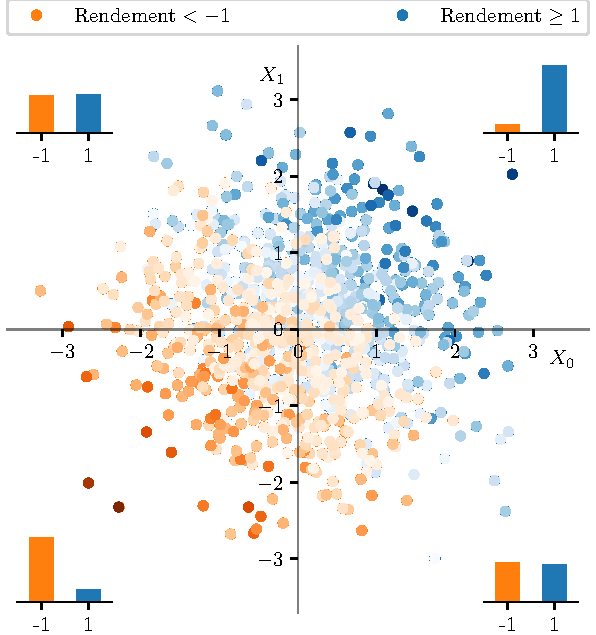
\includegraphics[width=\textwidth]{../experiments/fig/copula.pdf}
  \caption[Loi de marché]{Loi de marché théorique pour $\bar p = 2$. Les points bleus et
    rouges indiquent 500 réalisations d'une loi normale multivariée avec matrice de
    corrélation $\Sigma$. Les lois marginales Rademacher de la loi de marché entraînent un
    ``effondrement'' des réalisations en $\breve{X}_0$, $\breve{X}_1$ et $\breve{R}$ à
    leur signe. Les quatre histogrames présentent la distribution de $R$ par rapport à
    $X_0=\pm1$ et $X_1=\pm1$. On constate par ailleurs l'absence d'arbitrage d'une telle
    loi de marché puisqu'aucune région ne contient uniquement des rendements positifs ou
    uniquement des rendements négatifs.}
  \label{fig_copula}
\end{figure}


\begin{figure}[ht]
  \centering
  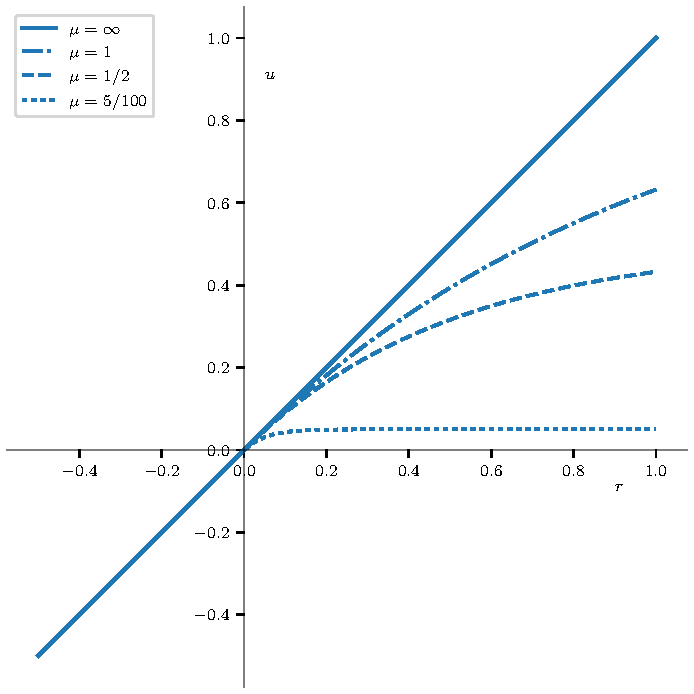
\includegraphics[width=\textwidth]{../experiments/fig/leus.pdf}
  \caption[Utilité Lipschitz exponentielle (LEU)]{Comportement des fonctions d'utilité
    exponentielles Lipschitz $\LEU_\mu$ selon le paramètre $\mu$. L'abscisse est l'axe des
    rendements, alors que l'ordonnée est celui des \textit{utils}. Le paramètre $\mu$ de
    chacune des instances $\LEU_\mu$ permet de quantifier l'aversion au risque : un
    paramètre $\mu\to\infty$ indique une attitude neutre au risque, alors qu'à l'autre extrême, un
    paramètre $\mu\to0$ modélise une indifférence (utilité constante) aux rendement
    positifs. Sur la branche négative, l'utilité correspond à la fonction identité, sur la
    branche positive, $\LEU_\mu(r) = \mu(1-e^{-r/\mu})$.}
  \label{fig_leus}
\end{figure}

\begin{figure}[ht]
  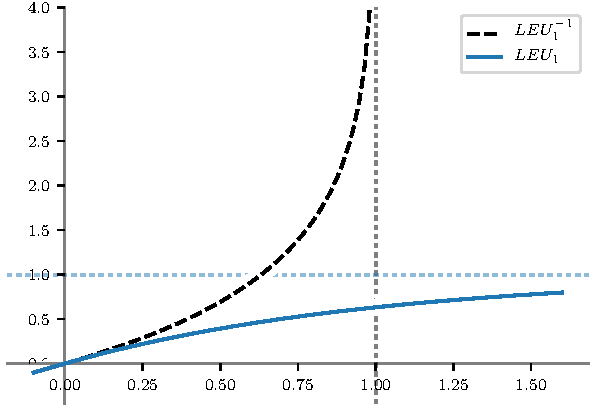
\includegraphics[width=\textwidth]{../experiments/fig/leu_inv.pdf}
  \caption[Fonction LEU et LEU inverse]{Utilité et utilité inverse. La fonction d'utilité
    permet de caractériser en \textit{utils} le rendement observé. L'\textit{util} est
    cependant une notion abstraite qu'on peut réexprimer en rendement à partir de la
    fonction utilité inverse. Une fonction $LEU_\mu(r)$ tend asymptotiquement vers $\mu$ à
    mesure que $r\to \infty$. Inversement, $LEU_\mu^{-1}(r)\to\infty$ à un rythme logarithmique lorsque
    $r\to\mu$. En effet, sur sa branche négative $\LEU_\mu^{-1}$ correspond à la fonction
    identité, alors que sur la branche négative, $\LEU_\mu^{-1}(r) = -\mu\log(1-r/\mu)$.}
  \label{fig_leu_inv}
\end{figure}

\clearpage


\subsection{\textit{n} variable, \textit{p} constant}
\label{emp:nvar}

L'objet de cette section est l'étude du cas canonique où la taille $n$ de l'ensemble
d'entraînement $\S_n$ augmente progressivement afin de donner une meilleure représentation
de $M$.


\subsubsection{Erreur de généralisation}

On rappelle tout d'abord que l'erreur de généralisation d'une politique d'investissement
$q$ consiste à mesurer la différence entre l'utilité (resp.~l'équivalent certain) espérée
observée en échantillon et l'utilité (resp.~l'équivalent certain) espérée hors
échantillon, ou, mathématiquement, de déterminer $\hEU(q) - \EU(q)$
(resp.~$\hCE(q) - \CE(q)$).

Avant de rentrer dans le vif du sujet, il peut être intéressant de voir graphiquement
comment se comportent différents quantiles de l'erreur de généralisation à mesure que de
nouveaux échantillons sont fournis à l'algorithme (\ie\ à mesure que $n$ augmente). La
Figure \ref{fig_genstats} illustre précisément ce comportement, en présentant l'erreur en
util et en rendement. Puisque la variable de rendement $R$ est bornée entre $-1$ et $1$ et
que son espérance marginale est nulle, le panneau b) indique qu'avec un échantillon
d'entraînement formé de $n=10$ observations de marché, l'erreur maximale sera d'environ
40\%. Par ailleurs, comme la courbe du 1\ier quartile correspond à une erreur nulle, on
peut conclure que dans environ 75\% des cas, la performance hors échantillon sera moindre
que celle observée en échantillon. Finalement, sans surprise, plus $n$ est élevé, moins
l'erreur de généralisation sera importante et tous ses quantiles finiront par converger
vers une erreur nulle. 


% La Table 1 indique par ailleurs le rythme de
% convergence des trois derniers quartiles d'erreur de généralisation en utilité. On
% constate que l'erreur médiane converge donc vers zéro presqu'à un rythme $\bigO(1/n)$
% alors que l'erreur maximale converge à un rythme près de $\bigO(n^{-1/2})$, donc plus
% lentement.


% \begin{table}[b]
%   \centering
%   \begin{tabular}{lSS[table-format = 1.3e1]}
%     \toprule
%     Quantile d'erreur & {Ordre de convergence} & \multicolumn{1}{c}{Erreur}\\
%     \midrule
%     Erreur maximale & -0.600 & 5.246e-03\\
%     75\ieme percentile d'erreur & -0.766 & 1.705e-03\\
%     Erreur médiane & -0.923 & 2.352e-03\\
%     \bottomrule
%   \end{tabular}
%   \caption{Ordre de convergence de chacun des trois derniers quartiles d'erreur de
%     généralisation (en util). L'erreur médiane converge donc vers zéro presqu'à un rythme
%     $\bigO(1/n)$ alors que l'erreur maximale converge à un rythme près de
%     $\bigO(n^{-1/2})$, donc plus lentement. Ce tableau a été produit à partir d'une
%     optimisation aux moindres carrés sur une fonction $an^k + b$, avec paramètres de
%     départ $b=0$, $a=1$ et $k=-1/2$.}
% \end{table}

La Figure \ref{fig_avrisk_gen} illustre quant à elle la relation entre l'aversion au
risque (caractérisée par le paramètre $\mu$ de la fonction d'utilité $\LEU$) et le 95\ieme
percentile d'erreur de généralisation en util et en équivalent certain. On constate en
particulier qu'une faible aversion au risque, toutes choses étant égales par ailleurs,
entraîne une plus grande erreur de généralisation. On peut expliquer cette observation
d'un point de vue géométrique, puisqu'une aversion plus prononcée au risque vient ajouter
de la courbure à la fonction d'utilité, et qu'en ce sens, cette courbure a le même effet
que l'ajout d'un terme de régularisation $\lambda\|q\|^2$ dans la fonction objectif de
l'algorithme. Or, comme l'idée même de la régularisation est de permettre d'établir des
politiques d'investissement plus conservatrices qui favorisent des investissement moins
importants, on comprend donc qu'une aversion au risque élevée aura le même genre d'effet
et entraînera donc une erreur hors échantillon moins importantes.

À la Figure \ref{fig_bound_errgen}, c'est le 95\ieme percentile d'erreur et sa borne
théorique $(\delta = 5\%)$ en fonction de $n$ qui sont illustrés, ce qui permet donc de
constater la pertinence des garanties théoriques offertes par l'algorithme
d'investissement. Ce qui frappe le plus, c'est surtout que la borne n'est pas exactement
serrée, les deux courbes différant l'une de l'autre d'un ordre de grandeur (soit d'un
facteur d'environ 10). Par exemple, il faut attendre d'avoir environ $n=150$ observations
avant de pouvoir garantir une erreur inférieure à 100\%, alors que le 95\ieme percentile
d'erreur empirique n'y est que de 5\%.

Néanmoins, il faut d'abord conserver à l'idée que ces bornes sont valides pour toute loi
de marché $M$ telle que $\xi\leq\sqrt{2}$ et $\rmax\leq 1$ et toute courbe d'utilité $u$ de
coefficient Lipschitz 1. C'est toutefois avec cette forme particulière de $M$ (marges
Rademacher) qu'on a pu observer les bornes plus serrées. Mais d'autre part, si les bornes
ne sont en tant que telles pas particulièrement fortes, l'ordre $\bigO(n^{-1/2})$ qu'elles
indiquent semble bien respecté empiriquement. Cette propriété est très importante
puisqu'elle permet à un investisseur de savoir de quelle façon et à quel rythme décroît
son risque d'erreur de généralisation en fonction de la taille de son ensemble
d'entraînement $\S_n$. 

Il peut en outre être intéressant de décomposer ce 95\ieme percentile d'erreur de
généralisation en sa composante de performance en échantillon $\hEU(\qh)$ et hors
échantillon $\EU(\qh)$ (Figure \ref{fig_bound_gencomps}). Cette figure permet de constater
que bien que la composante hors échantillon possède une utilité espérée positive, elle
sera cependant beaucoup plus faible que ce qui était anticipé par l'utilité espérée en
échantillon. De plus, la composante hors échantillon demeure relativement stable et c'est
la composante en échantillon qui converge vers elle. De plus, cette figure permet de
comprendre comment on peut passer d'une représentation en util à une représentation en
rendement suite à l'application de la fonction utilité inverse $\LEU^{-1}_\mu:\Ut \to \R$
(voir Figure \ref{fig_leu_inv}). Puisque $\mu=1$ ici, cette utilité inverse a un effet plus
prononcé pour des utilités proches de 1, et son effet décroit pour des utilités plus
faibles. Bien entendu, cette amplification est plus prononcée à mesure que l'investisseur
est averse au risque, ce qui dégrade alors la qualité des garanties offertes par
l'algorithme.


\newpage


\begin{figure}[h!]
  \centering
  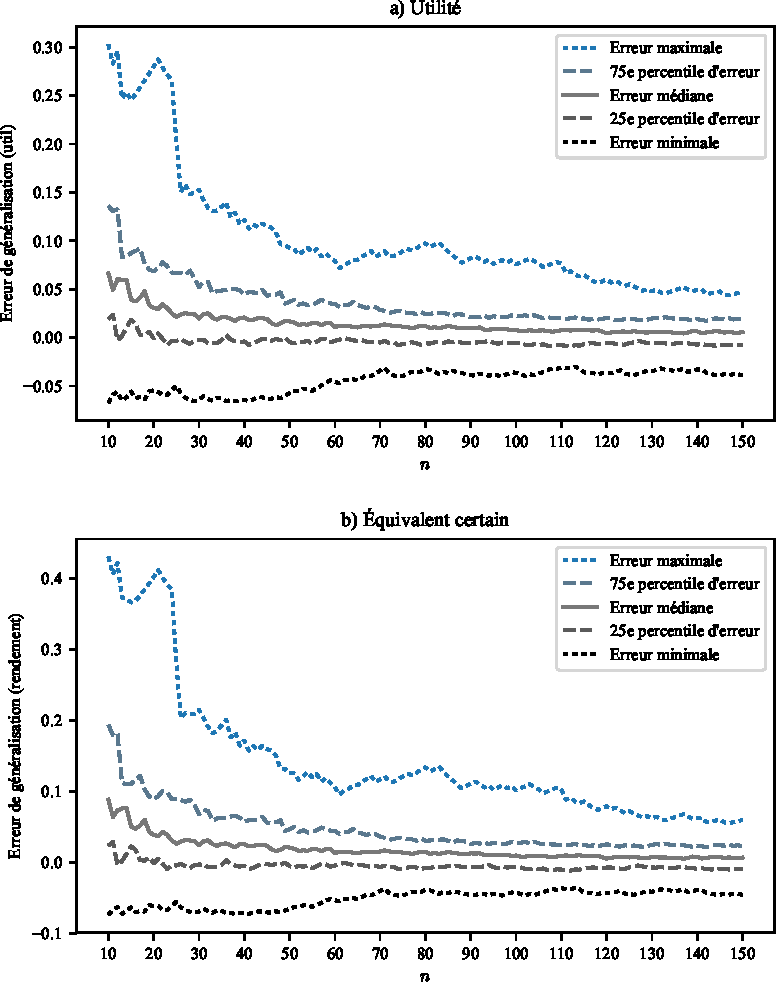
\includegraphics[width=\textwidth]{../experiments/fig/genstats.pdf}
  \caption[Quartiles de l'erreur de généralisation]{Progression des quartiles de l'erreur
    de généralisation en util et en équivalent certain en fonction de la taille $n$ de
    l'échantillonage. Dans environ 75\% des cas, la performance hors échantillon sera
    moindre que celle observée en échantillon. }
  \label{fig_genstats}
\end{figure}


\begin{figure}[h!]
  \centering
  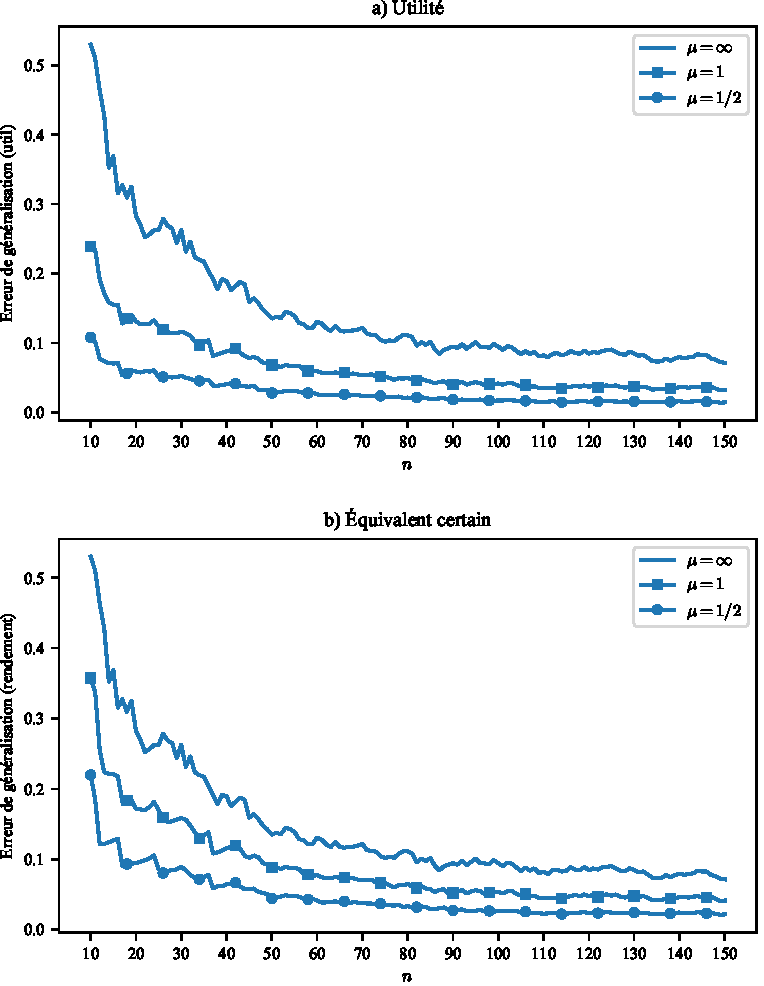
\includegraphics[width=\textwidth]{../experiments/fig/avrisk_gen.pdf}
  \caption[Aversion au risque et erreur de généralisation]{Progression du 95\ieme
    percentile d'erreur de généralisation en fonction de la taille de l'échantillon $n$
    pour trois niveaux d'aversion au risque. Plus l'aversion au risque est faible (avec
    comme cas limite l'attitude neutre au risque $\mu = \infty$), plus l'erreur de généralisation
    est importante, et inversement pour une forte aversion au risque. }
  \label{fig_avrisk_gen}
\end{figure}



\begin{figure}[h!]
  \centering
  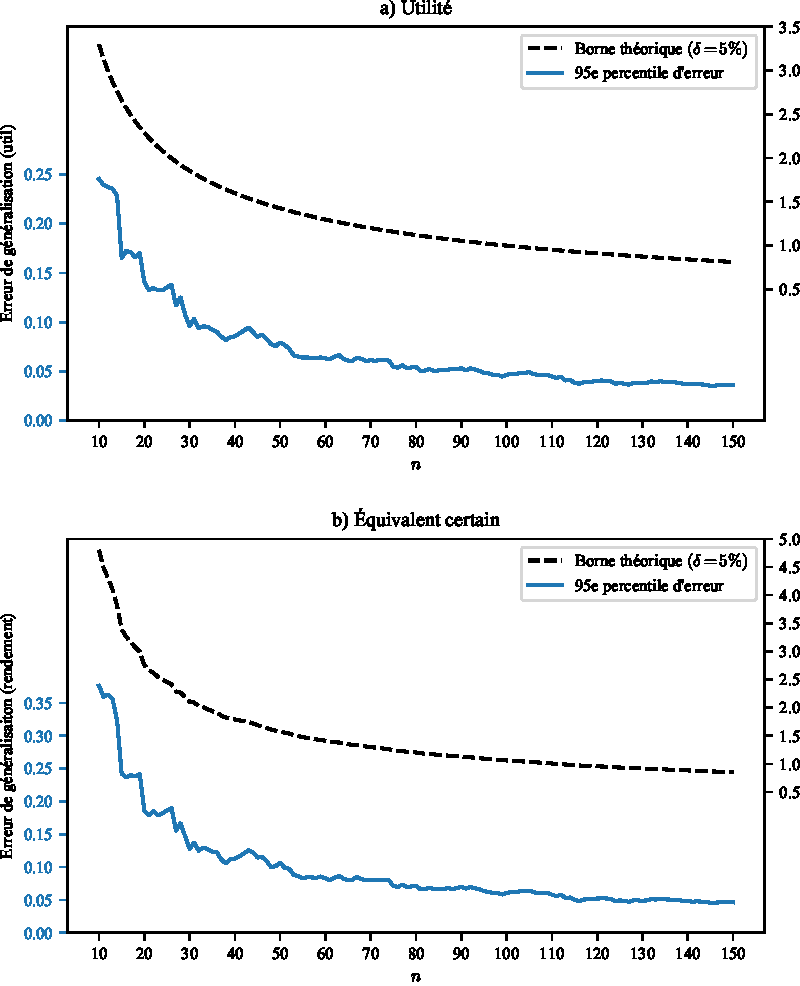
\includegraphics[width=\textwidth]{../experiments/fig/bound_errgen.pdf}
  \caption[Erreur de généralisation en fonction de $n$]{Progression du 95\ieme
    percentile l'erreur de généralisation et borne théorique (paramètre de confiance
    $\delta = 5\%$) en fonction de la taille d'échantillon $n$, exprimés en util et en
    rendement. Dû à la différence d'ordre, les deux figures font intervenir deux
    ordonnées: celle de gauche quantifie l'erreur empirique alors que celle de droite
    quantifie la borne théorique. Ainsi, la borne théorique est environ 10 fois supérieure
    à l'erreur empirique.}
  \label{fig_bound_errgen}
\end{figure}

\begin{figure}[h!]
  \centering
  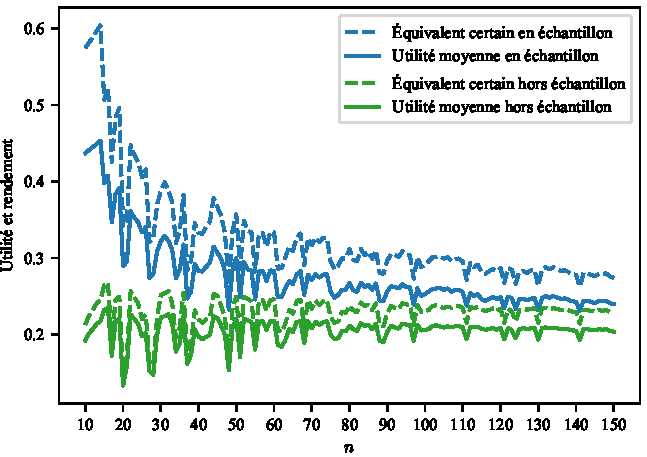
\includegraphics[width=\textwidth]{../experiments/fig/bound_gencomps.pdf}
  \caption[Composantes de l'erreur maximale]{Progression sur la même échelle des
    composantes de performance en échantillon et hors échantillon, exprimées en util et en
    rendement, du 95\ieme percentile d'erreur de généralisation de la Figure
    \ref{fig_bound_errgen} a). Plus une valeur d'utilité est grande, plus l'amplification
    de l'utilité inverse se fera ressentir. L'erreur de généralisation est donc plus
    importante lorsqu'elle est mesurée en unités de rendement qu'en unités d'utils.  }
  \label{fig_bound_gencomps}
\end{figure}

\clearpage


\subsubsection{Erreur de sous optimalité}

Contrairement à l'erreur de généralisation, l'erreur (en util) de sous optimalité
$\EU(\qs) - \EU(\qh)$ (resp.~$\CE(\qs) - \CE(\qh)$ dans le domaine des rendements) ne
bénéficie pas d'une convergence vers zéro du fait de la présence du terme de
régularisation dans l'algorithme $\alg(\S_n)$. En fait, la meilleure garantie offerte par
le Théorème \ref{thm3}, lorsque $n\to\infty$, correspond à $\lambda/2\|\qs\|^2$ dans le domaine des
utils.

Ainsi, la Figure \ref{fig_bound_errso} présente la progression du 95\ieme percentile de
l'erreur empirique de sous optimalité et de la borne théorique $\delta = 5\%$ selon la taille
$n$ de l'échantillon. En particulier, le facteur de régularisation constant $\lambda = 1$ fait
en sorte que, exprimés en utils, la borne théorique converge vers $\|q^\star\|^2/2$ (évaluée
numériquement à \num{3.16}) alors que le 95\ieme percentile d'erreur semble converger vers
une utilité espérée aux alentours de \num{0.24}.

D'autre part, la borne théorique de sous optimalité du 95\ieme percentile d'erreur
empirique est relâchée d'environ deux ordres de grandeur ($10^{-1}$ pour l'erreur
empirique \textit{vs} $10^{2}$ pour la garantie théorique). En fait, ce qui est
particulièrement déconcertant, c'est que même dans la limite $n\to\infty$, la borne théorique est
supérieure à la plus grande erreur empirique observée (\ie\ lorsque $n=10$)!  Cela étant,
même si la borne de sous optimalité est particulièrement relâchée, elle suggère en
revanche un ordre de convergence $\bigO(n^{-1/2})$ qui lui semble être en adéquation avec
le 95\ieme percentile de l'erreur de sous optimalité empirique.

Néanmoins, un investisseur ayant à cœur une faible erreur de sous optimalité devra
nécessairement faire converger son paramètre de régularisation vers zéro à mesure que de
nouvelles observations de la loi de marché sont disponibles. De plus, il a été démontré au
cours de la section précédente qu'on doit avoir $\lambda = \omega(1/\sqrt{n})$, \ie\ une décroissance
moins rapide que $\bigO(1/\sqrt{n})$ pour bénéficier d'une convergence vers une erreur
nulle. En particulier, si $\lambda = \bigO(n^{-k})$, alors la garantie théorique sera composée
de trois termes : $\bigO(n^{k-1}) + \bigO(n^{k-1/2}) + \bigO(n^{-k})$. Dans de telles
conditions, une constante $k=1/4$ semble bien adaptée pour balancer les deux derniers
termes.

Ainsi, la Figure \ref{fig_bound_errso3} présente la progression du 95\ieme percentile
d'erreur de sous optimalité empirique et de sa garantie théorique en fonction de $n$
lorsque $\lambda=(10/n)^{1/4}$. Ainsi défini, lorsque $n=10$, $\lambda$ est identique au facteur de
régularisation employé pour produire la Figure \ref{fig_bound_errso}. On constate
effectivement que l'erreur de sous optimalité est initialement la même pour les deux
figures. Cependant, alors qu'elle paraîssait stagner vers une erreur de 34\% avec une
régularisation constante, la décroissance $\lambda = \bigO(n^{-1/4})$ permet ici d'obtenir une
erreur de 26\% lorsque $n=150$. Par contre, il faut être bien conscient que la borne
théorique ne décroît plus qu'à un rythme $\bigO(n^{1/4})$.

\newpage

\begin{figure}[h!]
  \centering
  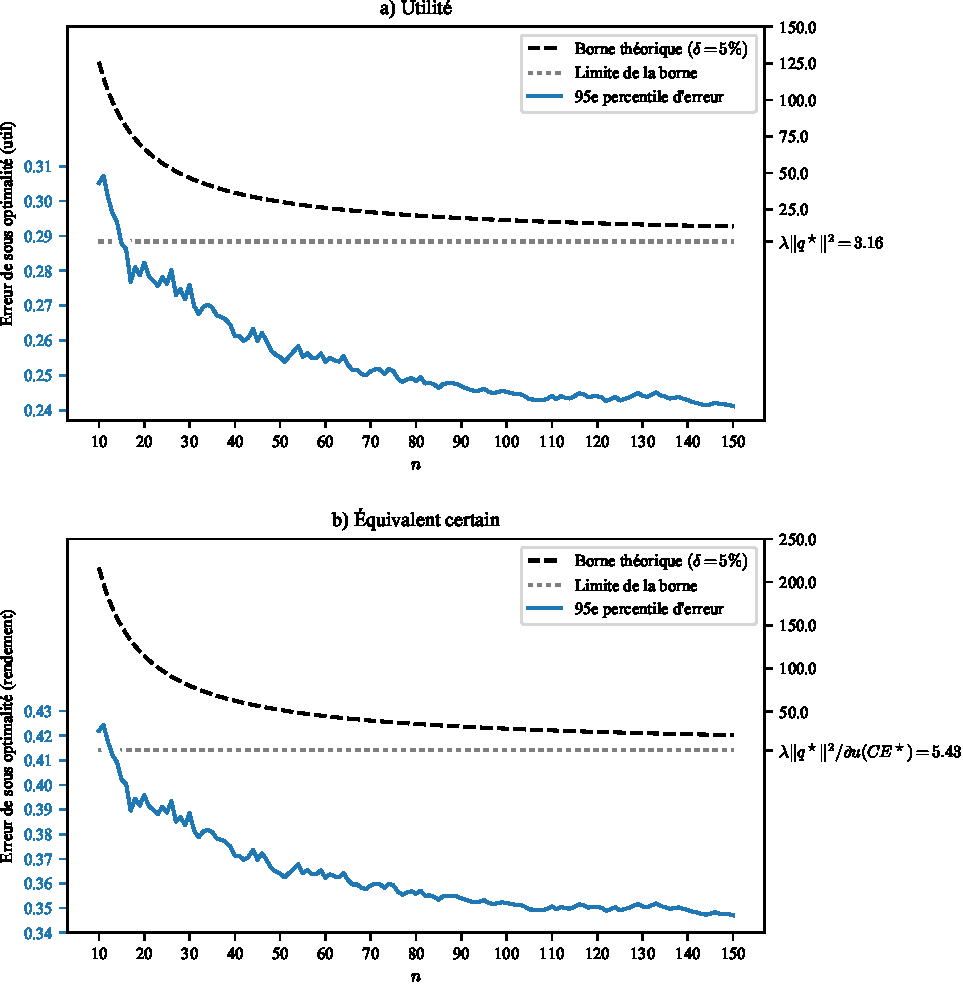
\includegraphics[width=1.3\textwidth]{../experiments/fig/bound_errso.pdf}
  \caption[Erreur de sous optimalité en fonction de $n$ ($\lambda$
  constant)]{Progression du 95\ieme percentile l'erreur empirique de sous optimalité et de
    la borne théorique $(\delta = 5\%)$ selon la taille $n$ de l'échantillonage. Le facteur de
    régularisation constant $\lambda = 1$ fait en sorte que, exprimés en utils, la borne
    théorique planche à $\lambda/2\|q^\star\|^2$ (évaluée numériquement à \num{3.16}) alors que le
    95\ieme percentile d'erreur semble plancher aux alentours de \num{0.24}. En plus
    d'être dégagée de près d'un ordre de grandeur de la courbe empirique, même la limite
    de la borne théorique est supérieure aux plus hautes valeurs observées. Cependant,
    l'ordre $\bigO(n^{-1/2})$ théorique se manifeste ici aussi dans le domaine empirique.}
  \label{fig_bound_errso}
\end{figure}

\begin{figure}[h!]
  \centering 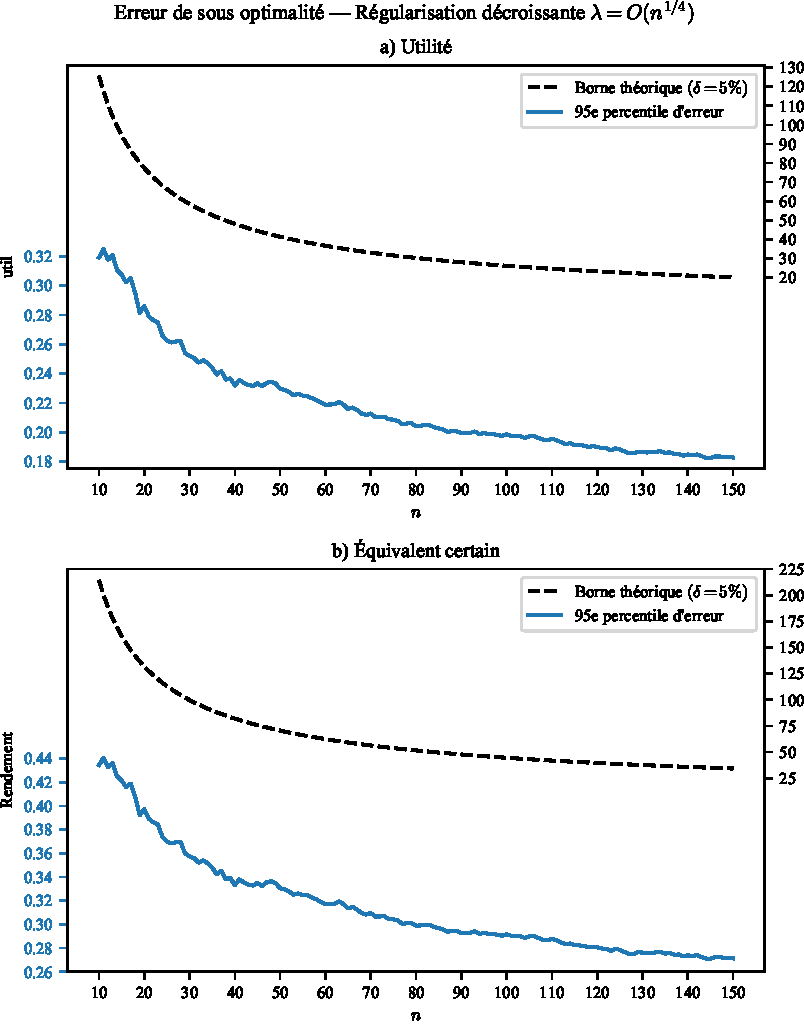
\includegraphics[width=\textwidth]{../experiments/fig/bound_errso3.pdf}
  \caption[Erreur de sous optimalité en fonction de $n$
  ($\lambda=\bigO(n^{-1/4})$)]{Progression du 95\ieme percentile de l'erreur de sous optimalité
    empirique exprimée en util et de la borne théorique $\delta=5\%$ selon la taille $n$ de
    l'échantillonage avec un facteur de régularisation $\lambda = (10/n)^{1/4}$. Le panneau a)
    indique la progression de la borne théorique alors que le panneau b) indique sa limite
    de la borne dans le cas $n\to\infty$. Contrairement au cas présenté à la Figure
    \ref{fig_bound_errso}, cette situation offre une garantie théorique d'une erreur nulle
    puisque le facteur de régularisation converge vers 0. Le rythme de convergence
    théorique n'est toutefois que de $\bigO(n^{-1/4})$.}
  \label{fig_bound_errso3}
\end{figure}


\clearpage

\subsection{\textit{n} constant, \textit{p} variable}
\label{emp:pvar}

Cette section sera consacrée à l'étude du rapport qu'entretient les erreurs de
généralisation et de sous-optimalité de notre algorithme lorsque sont incorporées à la
prise de décision de nouvelles variables de marché indépendantes des précédantes, tout en
conservant la taille d'échantillonnage constante.

On rappelle donc que les expériences suivantes dévoileront une à une les 50 variables de
marché $X_j$ à partir desquelles le rendement aléatoire $R$ est construit sur une copule
gaussienne. Trois situations différentes seront par ailleurs considérées, chacune d'elles
représentée respectivement par les vecteurs de corrélation
$\Corr(\tilde X,\tilde R) \in \Re^{\bar p}$ (dans le domaine de la copule gaussienne)
suivants:
\begin{gather}
  \rho = \left(\begin{matrix}\sqrt{\frac{1-\epsilon}{\bar p}} & \cdots & \sqrt{\frac{1-\epsilon}{\bar
          p}}\end{matrix}\right)\,;\\
  \rho = \left(\begin{matrix}\sqrt{1-\epsilon} & 0 & \cdots & 0\end{matrix}\right)\,;\\
  \rho = \left(\begin{matrix}0 & \cdots & 0\end{matrix}\right).
\end{gather}

La première situation sera donc celle où chacune des variables de marché a une influence
égale sur le rendement, la seconde celle où seule la première variable vient influencer la
réalisation du rendement et enfin la dernière celle où toutes les variables de marché sont
indépendantes au rendement, \ie\ elle ne forment qu'un ``bruit''. Ces trois situations
seront désignées respectivement par \textit{information dispersée}, \textit{information
  concentrée} et \textit{aucune information}.


\subsubsection{Erreur de généralisation}


La figure \ref{fig_pconst_infogen} présente donc pour ces trois situations comment
progresse leur 95\ieme percentile d'erreur de généralisation (avec $\bar n = 10$
observations du marché) et leur garantie théorique (ici commune aux trois cas) à mesure
que de nouvelles variables de marché sont dévoilées à l'algorithme. Intialement, lorsque
$p=1$ , la courbe \textit{Information concentrée} affiche sans surprise une erreur
beaucoup plus faible que les autres, puisque l'algorithme est déjà en mesure d'inférer la
meilleure politique d'investissement. Au contraire, la courbe \textit{Information
  dispersée} ne détecte qu'un faible lien entre cette variable de marché et $R$. À mesure
que de nouvelles varialbes sont dévoilée, la situation où l'information concentrée
continue de présenter une erreur plus faible aux autres cas, bien que la courbe d'erreur
dans la courbe \textit{Information dispersée} semble finir par la rejoindre. C'est de plus
lorsqu'aucune information n'est présente que le risque d'erreur de généralisation est le
plus grand, puisque toute décision d'investissement non nulle se traduit forcément par une
utilité hors échantillon plus faible qu'en échantillon.

En outre, la garantie sur l'erreur de généralisation, dans le cas d'un apprentissage par
noyau linéaire et d'une taille constante d'échantillonnage, suggère une progression de
l'erreur à un rythme linéaire $\bigO(p)$ (voir Section \ref{b:dim}). Or, les trois courbes
d'erreur empirique semblent indiquer qu'il se pourrait que ce ne soit que le cas que dans
une limite asymptotique, non observée dans ce cas ci. En effet, leur forme est loin d'être
linéaire et semble plutôt posséder une composante racine carrée. Il se pourrait donc que
le comportement de l'erreur de généralisation soit plutôt de $\bigO(p^{1/2}) + \bigO(p)$.

Afin de confirmer cette idée, la figure \ref{fig_pconst_infogen_cf} présente un ajustement
des 25 derniers points des trois courbes d'erreurs empiriques à deux fonctions
polynômiales $f(x) = a_0x + a_1x^{1/2} + b$ et $f(x) = a_0x^{1/2} + b$ par méthode des
moindres carrés. Il faut garder à l'esprit qu'estimer numériquement un ordre polynômial
n'est pas forcément simple, particulièrement lorsqu'on ne dispose que de si peu de points
($\bar p = 50$ dans ce cas-ci). Cela dit, dans les trois cas, l'hypothèse où l'erreur de
généralisation serait de nature $\bigO(p^{1/2}) + \bigO(p)$ semble plus convaincante
puisqu'elle suit de plus proche les vingt cinq premiers points des trois courbes. Cette
conclusion reste cependant spéculative.

\subsubsection{Sous optimalité}

Dans le cas où on ajoute de l'information, la sous optimalité, contrairement à l'erreur de
généralisation, peut référer à deux types d'erreur. Soit on compare la performance hors
échantillon de $\qh$ à celle de la politique optimale qui ne dispose que de
$p \leq \bar p$ variables d'information, soit à la politique optimale qui dispose des
$\bar p$ variables d'information nécessaires pour décrire $M$. Cependant, le développement
théorique qui a été mené au cours de la dernière section ne s'est implicitement préoccupé
que de la première situation.

La Figure \ref{fig_pconst_euinforelative} indique le comportement de l'utilité espérée
optimale $\nEU^\star$ en fonction du nombre de variables de marché connues de
l'algorithme. Naturellement, le cas où toute l'information est disponible dès $p=1$
affiche une utilité espérée optimale constante, alors qu'il s'agit plutôt d'une
progression à peu près linéaire lorsqu'on dévoile progressivement des variables
d'information chacunes faiblement corrélées à $R$, mais indépendantes l'une à
l'autre. Enfin, l'utilité espérée optimale est bien entendu nulle dans le cas où toutes
les variables de marché sont indépendantes à $R$.

La Figure \ref{fig_pconst_infosorelative} elle, indique la progression du 95\ieme
percentile des erreurs de sous optimalité des trois situations et de leur garantie
théorique pour $\delta = 5\%$ à mesure que de nouvelles variables de marché sont dévoilées à
l'algorithme, avec $\bar n = 10$ constant. Initialement, l'erreur de sous optimalité des
courbes \textit{Information dispersée} et \textit{Aucune information} est très faible
alors que la courbe \textit{Information concentrée} dispose déjà de suffisament
d'information pour permettre une erreur élevée. Puis, à mesure que $p$ se rapproche de
$\bar p$, on observe pour la courbe \textit{Information dispersée} une progression qui
correspond environ à la progression de l'utilité espérée optimale. Cela signifie donc que
l'erreur de sous optimalité serait maximisée lorsque l'utilité espérée hors échantillon
est nulle. Les deux autres courbes d'erreur empirique progressent beaucoup plus lentement,
possiblement à un rythme $\bigO(\sqrt{p})$. Dans le cas de la courbe \textit{Information
  concentrée}, puisque sa courbe de référence $\nEU^\star$ est constante, on en conclut
que l'utilité espérée hors échantillon minimale augmente selon $\bigO(\sqrt{p})$. 

De plus, le caractère linéaire annoncé n'est empiriquement pas très clair, sauf dans le
cas particulier où l'information est dispersée. Mais comme c'état le cas pour l'erreur de
généralisation, il n'est pas non plus impossible que l'erreur de sous optimalité ait un
ordre de progression $\bigO(\sqrt{p}) + \bigO(p)$: cela permettrait d'expliquer pourquoi
la courbe \textit{Information dispersée} est linéaire alors que les deux autres affichent
plutôt un caractère de progression racine carrée.
\newpage

\begin{figure}[h!]
  \centering
  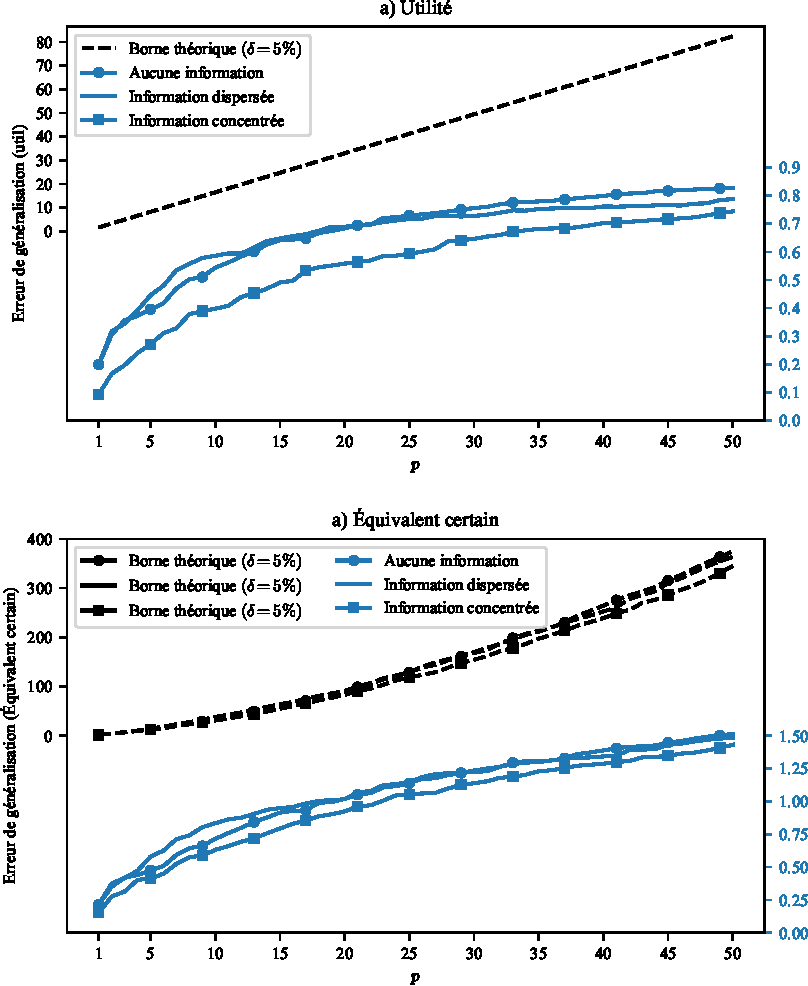
\includegraphics[width=1\textwidth]{../experiments/fig/pconst_infogen2.pdf}
  \caption[Erreur de généralisation en fonction de $p$]{Progression du 95\ieme percentile
    de l'erreur de généralisation exprimée en util et en équivalent certain à mesure que
    de nouvelles variables de marché sont dévoilées à l'algorithme, pour une taille
    d'échantillonnage constante $\bar n = 10$. Dans le domaine des utils, illustré par le
    panneau a), la borne théorique est commune aux trois situations et progresse
    linéairement. Lorsque $p=1$, la courbe \textit{Information concentrée} affiche sans
    surprise une erreur initialement plus faible que les autres, puisque l'algorithme est
    déjà en mesure d'inférer la meilleure politique d'investissement. Les courbes
    \textit{Aucune information} et \textit{Information dispersée} présentent une erreur
    similaire lorsque $p$ est faible (donc peu de variables connues) mais se distancent
    l'une de l'autre à mesure que $p$ converge vers $\bar p$.}
  \label{fig_pconst_infogen}
\end{figure}

\begin{figure}[h!]
  \centering
  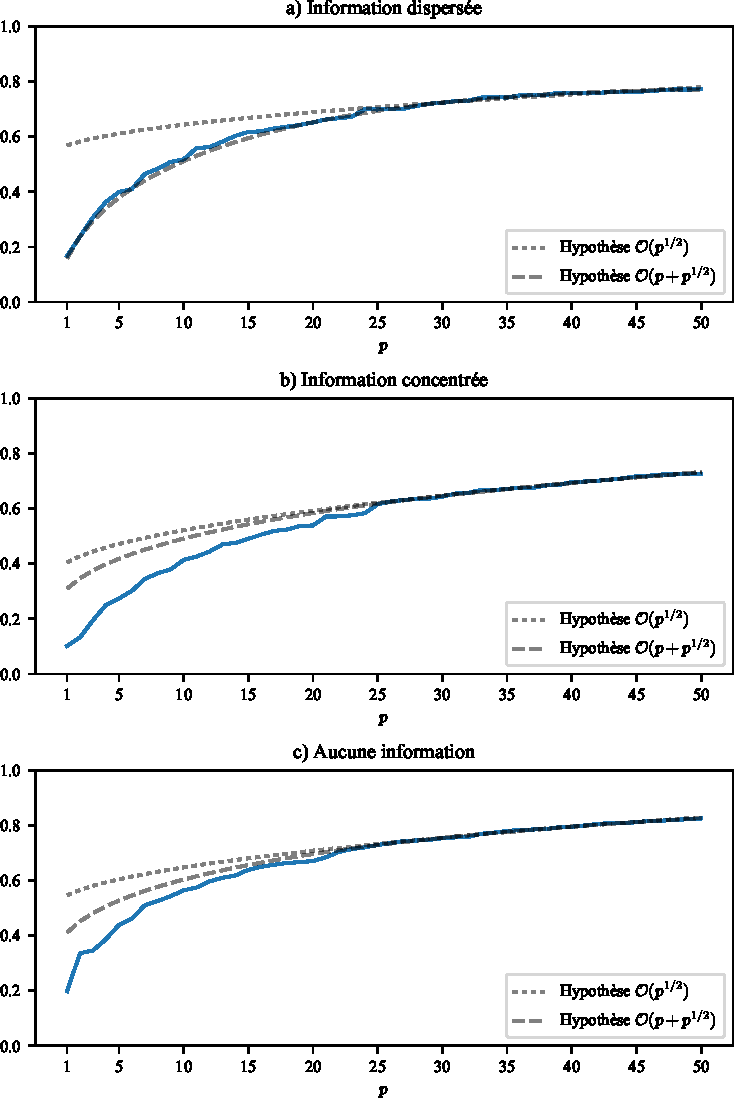
\includegraphics[width=1\textwidth]{../experiments/fig/pconst_infogen_cf.pdf}
  \caption[Ajustement des courbes d'erreurs de généralisation]{Ajustement des 25 derniers
    points des courbes d'erreur présentées à la Figure \ref{fig_pconst_infogen} à deux
    polynômes $f(p) = a_0p + a_1 p^{1/2} + b$ et $f(p) = a_0p + b$. Entre les deux,
    l'hypothèse où l'erreur aurait une progression $\bigO(p^{1/2}) + \bigO(p)$ serait
    ainsi la plus probable.}
  \label{fig_pconst_infogen_cf}
\end{figure}

\clearpage




\begin{figure}[h!]
  \centering
  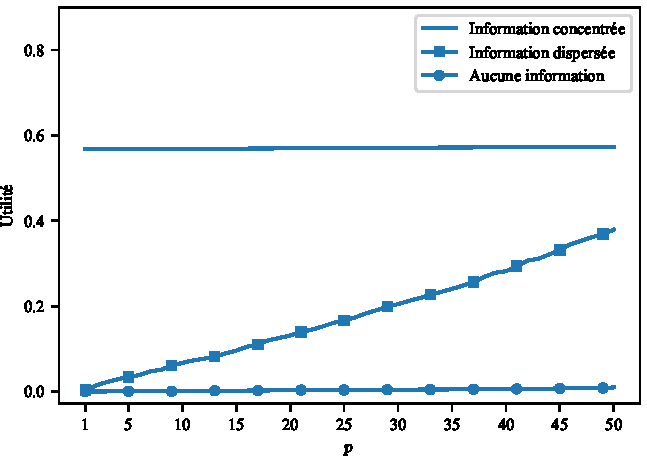
\includegraphics[width=\textwidth]{../experiments/fig/pconst_euinforelative.pdf}
  \caption[Utilité espérée optimale en fonction de $p$]{Progression de l'utilité espérée
    optimale $\nEU^\star$ en fonction du nombre de variables de marché connues. Naturellement,
    le cas où toute l'information est disponible dès $p=1$ affiche une utilité espérée
    optimale constante, alors qu'il s'agit plutôt d'une progression à peu près linéaire
    lorsqu'on dévoile progressivement des variables d'information chacunes faiblement
    corrélées à $R$, mais indépendantes l'une à l'autre. Enfin, l'utilité espérée optimale
    est bien entendu nulle dans le cas où toutes les variables de marché sont
    indépendantes à $R$. Les bornes théoriques exprimées en util se confondent car elles
    sont numériquement très rapprochées.}
  \label{fig_pconst_euinforelative}
\end{figure}

\begin{figure}[h!]
  \centering
  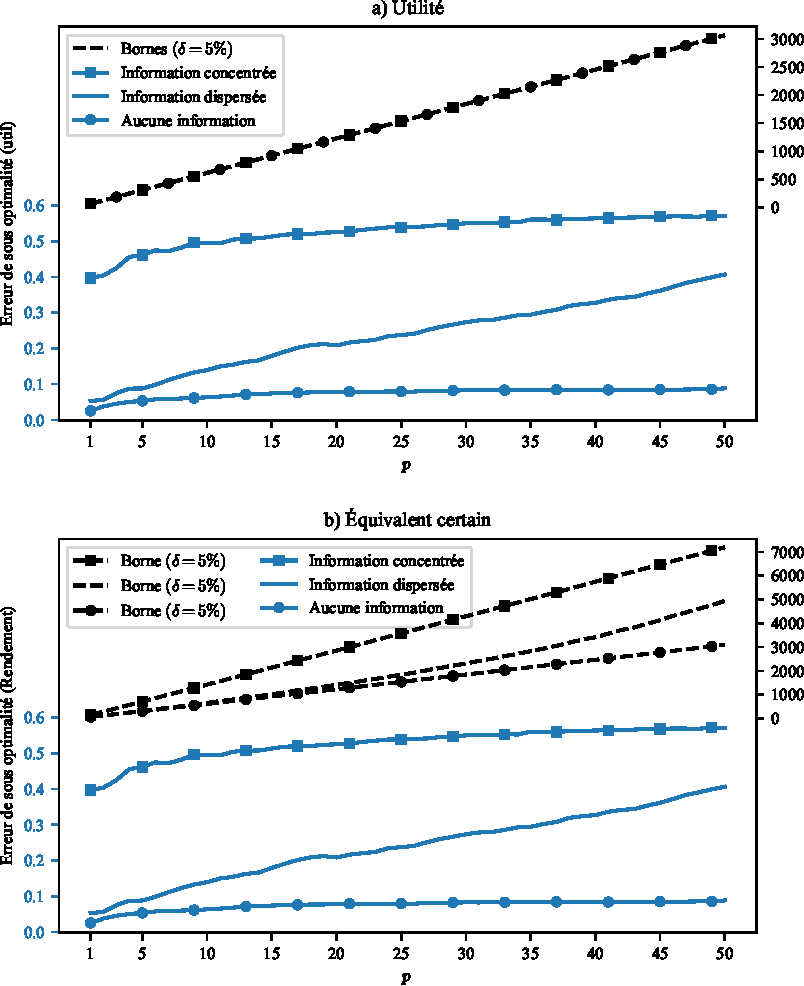
\includegraphics[width=\textwidth]{../experiments/fig/pconst_so.pdf}
  \caption[Erreur de sous optimalité en fonction de $p$]{Progression du 95\ieme percentile
    des erreurs de sous optimalité et de leur garantie théorique à mesure que de nouvelles
    variables de marché sont dévoilées à l'algorithme, avec $\bar n = 10$
    constant. Initialement, l'erreur de sous optimalité des courbes \textit{Information
      dispersée} et \textit{Aucune information} est très faible alors que la courbe
    \textit{Information concentrée} dispose déjà de suffisament d'information pour
    permettre une erreur élevée. Puis, à mesure que $p$ se rapproche de $\bar p$, on
    observe pour la courbe \textit{Information dispersée} une progression linéaire, alors
    que l'erreur plafonne dans les deux autres cas. Les garanties en util donnent une
    progression qui elle est linéaire en util. }
  \label{fig_pconst_infosorelative}
\end{figure}


\clearpage

\subsection{\textit{n} et \textit{p} variables}
\label{emp:npvar}

Finalement, cette section cherche à illustrer le comportement de l'erreur de
généralisation et de sous optimalité lorsqu'on est en présence de régimes dynamiques entre
$n$ et en $p$, \ie\ lorsque $p=\bigO(n^k)$. Trois régimes seront étudiés : celui où
$p=\bigO(n^{1/2})$, $p=\bigO(n^{3/4})$ et $p=\bigO(n)$. La façon de procéder restera la
même que celle employée aux sections précédentes. Les percentiles d'erreur seront
déterminés à partir d'un échantillon formé de $m=150$ ensembles d'entraînement de taille
$n$, $n$ variant de 9 à 50. Le nombre de variables de marché dévoilées sera ensuite donné
à partir d'une des trois relations suivantes : $p=2n$, $p=3.5n^{3/4}$ et $p=6n^{1/2}$,
selon le régime. Le marché sera constitué de $\bar p = 100$ variables, ce qui correspond à
$p(\bar n)$ dans le régime $p = \bigO(n)$. Ces relations ont été déterminées afin que les
valeurs initiales de $p$ soient identiques et qu'elles conservent le même ordre de
grandeur sur toute l'expérience (voir Figure \ref{fig_np_np}).

\begin{figure}[h]
  \centering
  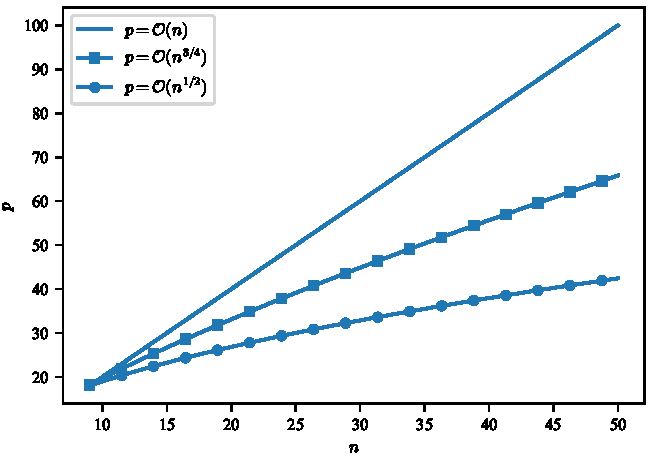
\includegraphics[width=0.7\textwidth]{../experiments/fig/np_np.pdf}
  \caption[Progression des trois régimes $p=\bigO(n^{1/2}),\bigO(n^{3/4}),\bigO(n)$]{En
    fonction de $n$, trois de cas de figure seront étudiés où le nombre $p$ de variables
    de marché dévoilées à l'algorithme dépend de $n$. Dans les expériences de cette
    section, $n$ variera de $9$ à $50$. La relation entre $p$ et $n$ sera alors
    respectivement donnée par $p = 2n$, $p=3.5n^{3/4}$ et $p=6n^{1/2}$.}
  \label{fig_np_np}
\end{figure}


Les propriétés mathématiques des deux types d'erreur établies à la Section \ref{b:dim}
suggérait un ordre asymptotique $\bigO(p\,n^{-1/2})$. Les résultats empiriques de la Section
\ref{emp:nvar} (\textit{n} variable, \textit{p} constant) ont d'abord permis de confirmer
l'ordre $\bigO(1/\sqrt{n})$ avec $p$ constant. Puis à la Section \ref{emp:pvar}
(\textit{n} constant, \textit{p} variable), la progression qu'on aurait pu anticiper être
linéaire s'est révélée comporter possiblement une composante racine carrée, \ie\
$\bigO(p) + \bigO(\sqrt{p})$. Ainsi, uniquement à partir de ces observations, on pourrait
conjecturer que l'erreur se comporte en fait comme
$\bigO(p/\sqrt{n}) + \bigO(\sqrt{p/n})$. Du fait de la dominance de $1/\sqrt{n}$ sur
$1/n$, rien n'empêcherait non plus que l'ordre soit $\bigO(p/n) + \bigO(\sqrt{p/n})$.


\subsubsection{Erreur de généralisation}


La Figure \ref{fig_bound_npgenu} présente la progression du 95\ieme percentile de l'erreur
de généralisation et de la garantie théorique ($\delta = 5\%$) des trois régimes de $p$ en
fonction de la taille d'échantillonage $n$. Ce qui frappe surtout, c'est comment les
ordres théoriques n'ont rien à voir avec les ordres empiriques. Soit par exemple le cas où
$p=\bigO(\sqrt{n})$. La courbe de la garantie demeure constante alors qu'en fait c'est
plutôt une décroissance qui est observée. Si on a plutôt une progression $p=\bigO(n)$, il
aurait été raisonnable de penser que l'erreur de généralisation augmenterait, alors que
même dans ce cas, elle continue de décroître!

La Figure \ref{fig_np_np32} présente le 95\ieme percentile de l'erreur de généralisation
suivant un autre régime où $p=0.0016n^{3/2}$. Si l'erreur est alors bien croissante, il
faut être prudent et éviter de généraliser cette observation puisque la valeur de départ
$p = 1$ lorsque $n=9$ n'est pas la même que pour les trois régimes de la Figure
\ref{fig_bound_npgenu} où $p=18$ lorsque $n=9$. Mais de toute façon, les résultats de la
Section \ref{emp:pvar} confirment qu'il existe un point où si $p$ domine suffisament $n$
l'erreur de généralisation devra croître. Il n'est cependant pas clair quel est ce point,
ni comment il dépend de $n$ ou de $p$.


\subsubsection{Erreur de sous optimalité}

La Figure \ref{fig_bound_npgsou} présente quant à elle la progression du 95\ieme
percentile de l'erreur de sous optimalité de la borne de généralisation selon les trois
régimes à l'étude, $p=\bigO(n^{1/2}),p=\bigO(n^{3/4})$ et $p=\bigO(n)$. L'ordre
$\bigO(p/\sqrt{n})$ de la borne théorique semble ici respecté, puisque l'erreur de sous
optimalité demeure constante dans le cas $p=\bigO(\sqrt{n})$, alors qu'elle augmente dans
les deux autres cas. Cependant, les courbes théoriques décroissent, excepté lorsque
$p=\bigO(n)$!

Pour expliquer ce phénomène contre intuitif, il suffit de réaliser que la borne théorique
a en fait une croissance $\bigO(p/\sqrt{n}) + \bigO(\sqrt{p/n}) + \bigO(1)$. Donc si
$p=\bigO(\sqrt{n})$, l'ordre asymptotique de l'erreur sera alors $\bigO(1)$, \ie\ constant
mais le deuxième terme forcera une décroissance $\bigO(\sqrt{n})$ vers cette constante, et
c'est précisément cette décroissance qu'on observe dans la Figure \ref{fig_bound_npgsou}.

De plus, il ne faut pas oublier que la norme de la décision optimale
$\lambda\|q^\star\|^2$ entre aussi dans la composition de la borne théorique, et donc possiblement
dans celle de l'erreur empirique de sous optimalité. Hélas, l'ordre de grandeur de cette
décision optimale est inconnue.

Cette figure illustre en fait assez bien le problème à réduire la progression des erreurs
en ordres asymptotiques. En effet, si l'erreur est polynômiale, alors même si un certain
ordre doit émerger asymptotiquement, lorsque $n$ est fini, il est tout à fait possible que
ce soit un terme d'un autre ordre qui domine la progression.  Avec les paramètres choisis
pour l'expérience de la Figure \ref{fig_bound_npgsou}, si l'ordre de l'erreur de sous
optimalité est effectivement de $\bigO(p/\sqrt{n}) + \bigO(\sqrt{p/n})$, alors il est
clair que seule la première composante joue sur la progression de l'erreur. À la Section
\ref{emp:pvar} où le cas où $n$ étant constant était étudié, il semblait pourtant que
l'erreur progresse en $\bigO(\sqrt{p}) + \bigO(p)$, ce qui laisse donc finalement assez
incertain l'ordre véritable de l'erreur de sous optimalité.


\begin{figure}[h!]
  \centering
  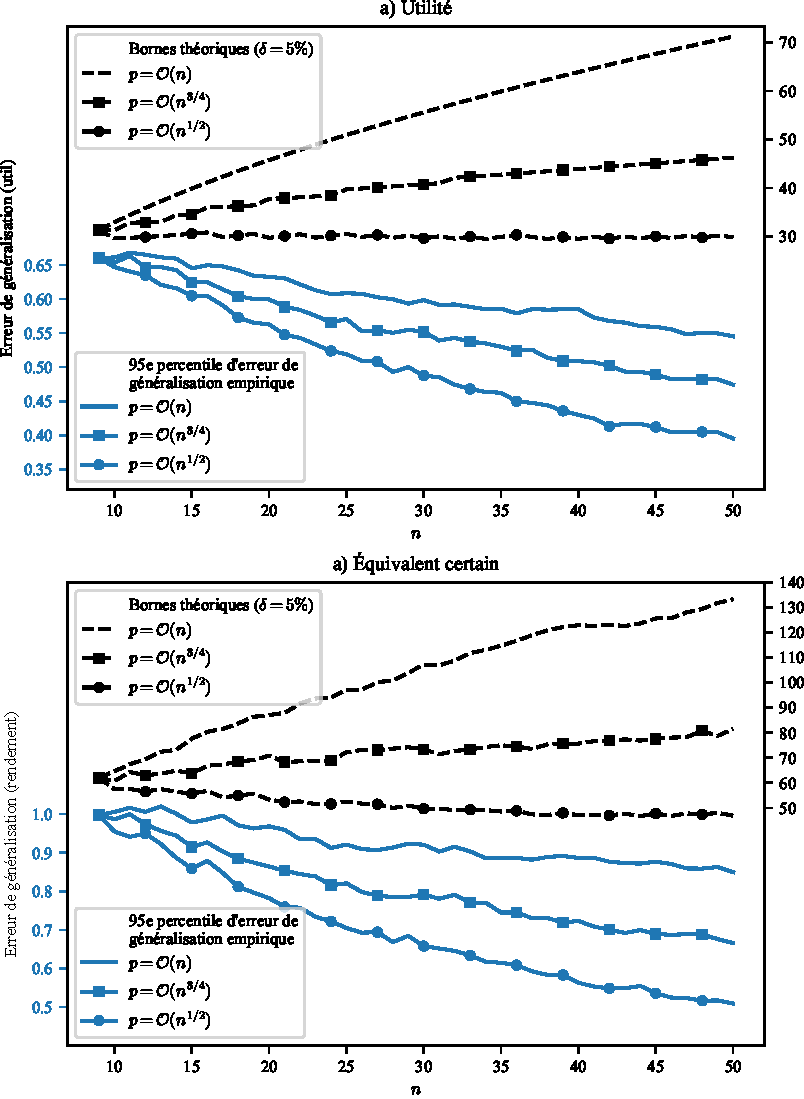
\includegraphics[width=\textwidth]{../experiments/fig/bound_npgenu.pdf}
  \caption[Erreur de généralisation -- Régimes $p=\bigO(n^{1/2}),\bigO(n^{3/4}),\bigO(n)$]
  {Progression du 95\ieme
    percentile d'erreur de généralisation et des garanties théorique en fonction de $n$,
    selon le régime de $p$. Une forte disparité entre la courbe des garanties théoriques
    et celle de l'erreur empirique est observée. Les courbes théoriques suggérant une
    progression de l'erreur $\bigO(p/n^{1/2})$, on se serait attendu à une amplification
    de l'erreur dès que $p$ domine $n^{1/2}$, \ie\ si $p=\omega(n^{1/2})$. Pourtant, cette
    figure indique que même si $p$ est de l'ordre de $n$, \ie\ $p = \bigO(n)$, l'erreur de
    généralisation empirique décroit tout de même.  }
  \label{fig_bound_npgenu}
\end{figure}

\begin{figure}[h!]
  \centering
  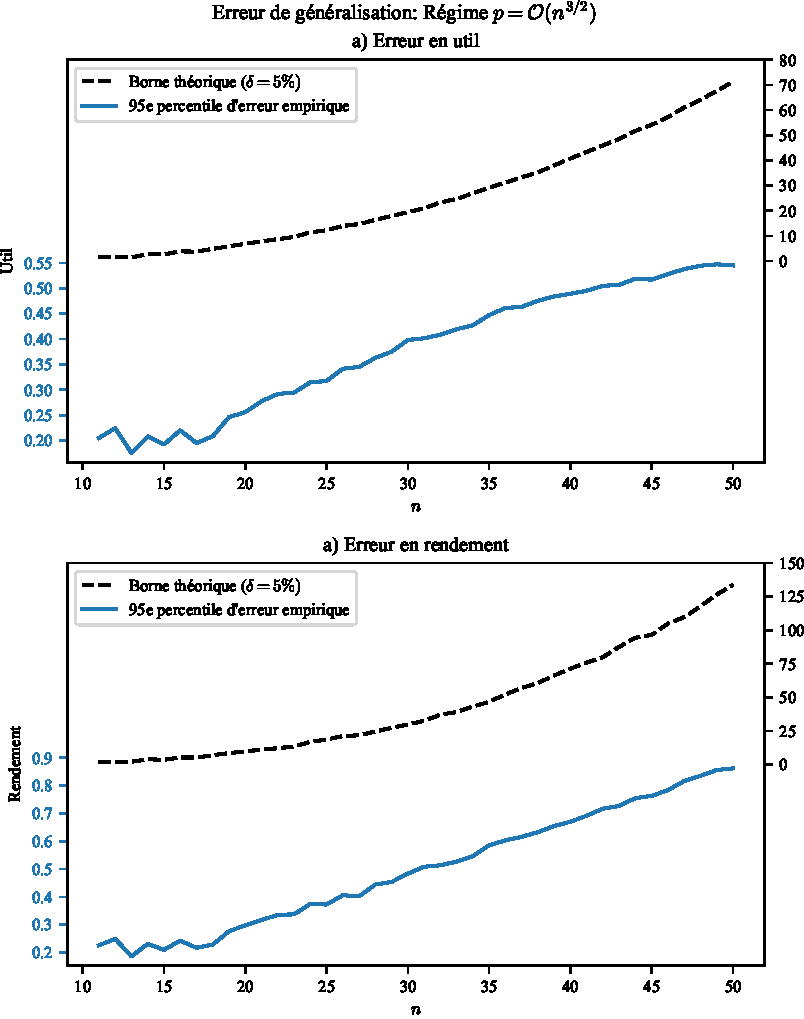
\includegraphics[width=\textwidth]{../experiments/fig/bound_np_np32.pdf}
  \caption[Erreur de généralisation -- Régime $p=\bigO(n^{3/2})$]{Progression du 95\ieme
    percentile de l'erreur de généralisation et de sa borne théorique $(\delta = 5\%)$ en
    fonction de la taille de l'échantillonage $n$. La relation entre $n$ et $p$ est donnée
    par la partie entière de $p = 0.0016n^{3/2}$. On observe bien une croissance de
    l'erreur de généralisation, cependant il serait trompeur de comparer ce résultat à
    celui présenté à la Figure \ref{fig_bound_npgenu} puisque le nombre $p$ de variables
    de marché est initialement beaucoup moins élevé dans ce cas-ci.}
  \label{fig_np_np32}
\end{figure}

\begin{figure}[h!]
  \centering
  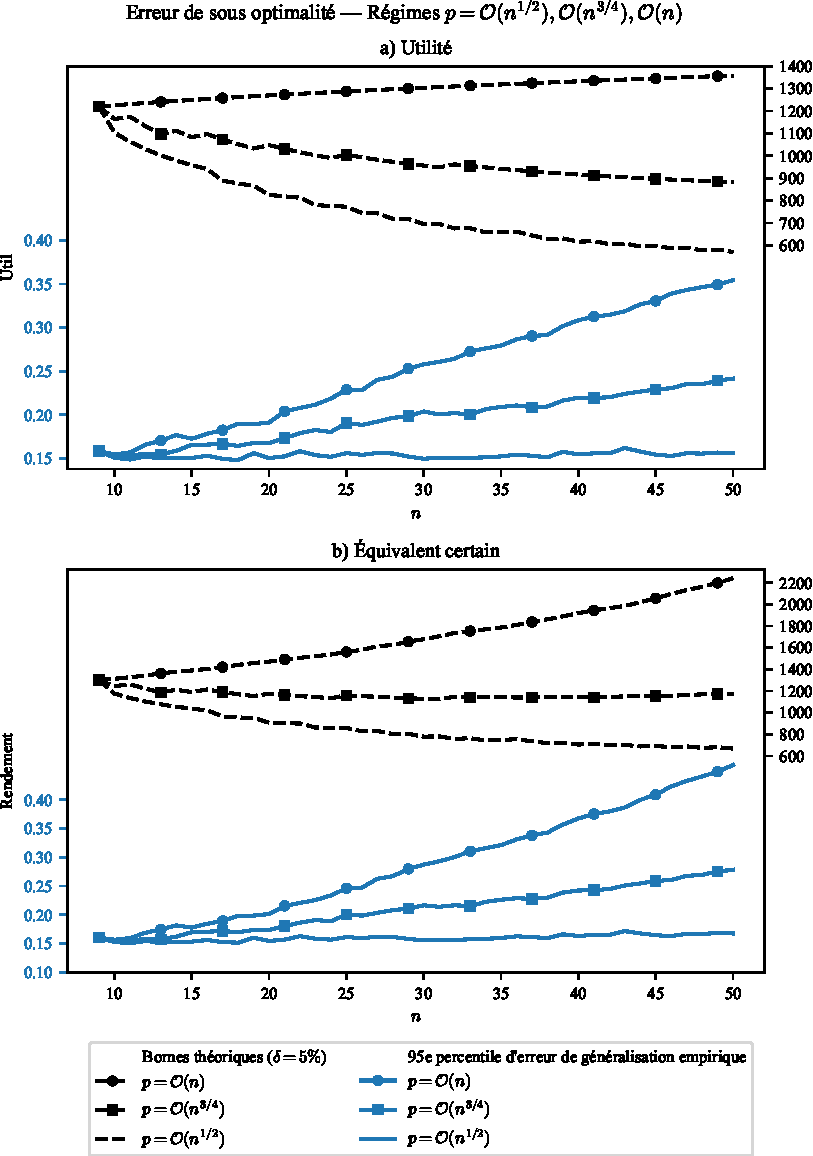
\includegraphics[width=\textwidth]{../experiments/fig/bound_test.pdf}
  \caption[Erreur de sous optimalité -- Régimes $p=\bigO(n^{1/2}),\bigO(n^{3/4}),\bigO(n)$]
  {Progression du 95\ieme percentile de l'erreur de sous optimalité et de sa garantie
    théorique $(\delta=5\%)$ selon les trois régimes à l'étude,
    $p=\bigO(n^{1/2}),p=\bigO(n^{3/4})$ et $p=\bigO(n)$. L'ordre $\bigO(p/\sqrt{n})$ de la
    borne semble ici respecté, puisque l'erreur de sous optimalité demeure constante dans
    le cas $p=\bigO(\sqrt{n})$, alors qu'elle augmente dans les deux autres
    cas. Cependant, les courbes théoriques décroissent, excepté lorsque $p=\bigO(n)$!}
  \label{fig_bound_npgsou}
\end{figure}

\clearpage

\subsection{Conclusion}

Cette section a permis d'illustrer le comportement des erreurs de généralisation et de
sous optimalité dans un cas relativement simple, où l'algorithme de décision ne disposait
que d'un noyau linéaire et où les variables de marché et le rendement étaient toutes
distribuées selon une loi Rademacher, liées les unes autres par une copule gaussienne.

Il a pu être établi assez clairement que pour un nombre constant de variables de marché,
l'erreur décroît bien à un rythme $\bigO(1/\sqrt{n})$, ce qui d'une certaine façon est
sans surprise au su du théorème limite centrale ou de la théorie de la programmation
stochastique (voir \cite{shapiro2009lectures}).

Les choses se compliquent sensiblement lorsqu'on fait intervenir un nombre croissant de
variables de marché. Néanmoins, avec $n$ constant, les expériences menées plus haut ont
permis de constater que l'ordre des deux types d'erreur est probablement $\bigO(p)$, bien
que ce régime puisse mettre du temps à apparaître et qu'il serait en fait plus précis de
parler d'un régime $\bigO(p) + \bigO(\sqrt{p})$.

La théorie par contre ne permet pas d'expliquer les courbes d'erreur de généralisation
observées dans des régimes dynamiques où $p=\bigO(n^k)$, où, pour $k\leq1$, celles-ci étaient
toutes décroissantes alors qu'elles auraient dû être croissantes. Ceci dit, l'étude faite
sur l'erreur de sous optimalité viendrait supporter l'idée que sa progression serait bien
de $\bigO(p/\sqrt{n})$. 




%%% Local Variables:
%%% mode: latex
%%% TeX-master: "memoire"
%%% End:

\section{Conclusion}

SVM multiclasse

Time series et learning


%%% Local Variables:
%%% mode: latex
%%% TeX-master: "main_conclusion"
%%% End:

\section{Appendix}

\subsection{Proof of Theorem \ref{thm:outsampleBound1}}

In this proof, we will employ a theorem made famous by Bousquet-Ellisseef to analyse relevant asymptotic statistical properties of the following estimator.
\begin{definition}
Let $\qhatOp:\Re^{(p+1)\times n}\rightarrow \Re^p$ be the procedure that generates the optimal solution of problem \eqref{EUFhatReg} based on a sample set $\{(x_i^1,r_i^1)\}_{i=1}^n$. 
\end{definition}

We start by presenting two lemmas that establish some important properties of problem \eqref{EUFhatReg}. 
\begin{lemma}\label{beta-bound}
  When assumptions \ref{ass:R} and \ref{ass:u}  are satisfied, the estimator $\bold{\qhat}(\cdot)$ has $\beta$-stability with $ \beta = \frac{(\gamma\bar r\xMax)^2}{2\lambda n}$. Namely, for any two sample sets $\Sn^1:=\{(x_i^1,r_i^1)\}_{i=1}^n$ and $\Sn^2:=\{(x_i^2,r_i^2)\}_{i=1}^n$ that are exactly identical except for the $j$-th sample, i.e., $(x_i^1,r_i^1)=(x_i^2,r_i^2)$ for all $i\neq j$, the following holds:
  \[
    |u(r\,\qhatOp(\Sn^1)^T x) - u(r\,\qhatOp(\Sn^2)^T x)| \leq \beta\,,\,\forall\,x\in\Sx\,,\,\forall\,r\in\Sr\;.
  \]
\end{lemma}
\begin{proof}
First, following the terminology presented in   \cite{bousquet2002stability} (see Definition 19), we can establish that $\qhatOp(\cdot)$ has $\sigma$-admissibility of $\gamma\bar{r}$. This is simply done by exploiting the fact that $\Sr$ is bounded and that $u(\cdot)$ is Lipschitz continuous. The detailed derivations consider that for any pair $(q_1,q_2)\in\Re^p\times\Re^p$, one has that
\[ |u(r\,q_1^T x) - u(r\,q_2^T x)| \leq \gamma |rq_1^Tx - rq_2^Tx|\leq \gamma\bar{r}\ |q_1^Tx - q_2^Tx| \,,\,\forall\,r\in\Sr\,,\,\forall\,x\in\Sx\;.\]
 The $\beta$-stability of $\bold{\qhat}(\cdot)$ then follows directly from Theorem 22 in \cite{bousquet2002stability}.
\end{proof}

\begin{lemma}  \label{u-bound}
  When assumptions \ref{ass:R}, \ref{ass:X} and \ref{ass:u}  are satisfied, the amount of utility attained by implementing the investment strategy characterized by $\qhatOp(S_n)$ is bounded by
\[|u(R\,\qhatOp(\Sn)^TX)|\leq \frac{\gamma^2\xi^2 \bar{r}^2}{2\lambda}\;\mbox{with probability $1$.}\]  
\end{lemma}

\begin{proof}
This proof relies mostly on demonstrating that $\qhatOp(\Sn)$ is bounded with probability one. Indeed, when this is the case, then we have that 
\[ u(R\,\qhatOp(\Sn)^T X) \leq u(0) + \gamma | R\qhatOp(\Sn)^TX| \leq \gamma\bar{r}\xi \|\qhatOp(\Sn)\|\;\mbox{with probability $1$.}\]
In order to show that $\qhatOp(\Sn)$ is bounded, we reformulate problem \eqref{EUFhatReg} as follows
  \begin{eqnarray*}
  \maximize_{s\in\Re,v\in\Re^p} && \frac{1}{n}\sum_{i=1}^n u(s R_i\,X_i^T v) - \lambda s^2\\
\st&& s\geq0\;,\;\|v\|=1\;,
  \end{eqnarray*}
such that $\qhatOp(\Sn) =s^*\cdot v^*$ when $(s^*,v^*)$ is the pair of optimal assignments for this optimization problem. It is therefore clear that $s^*=\|\qhatOp(\Sn)\|$ and our proof reduces to establishing an upper bound for $s^*$.  By recognizing that $s^*=\argmax_{s\geq 0} g(s):=\frac{1}{n}\sum_{i=1}^n u(s R_i\,X_i^T v^*) - \lambda s^2$ and that $g(s)$ is a concave function, then it is necessarily the case that if there exists a $\bar{s}\geq 0$ such that $g(\cdot)$ is non-increasing at $\bar{s}$ then $s^* \leq \bar{s}$. We can actually show that this is the case for $\bar{s}:= \gamma\bar{r}\xi/(2\lambda)$ by upper bounding the impact of taking a step of $\Delta>0$: 
\begin{eqnarray*}
g(\bar{s}+\Delta)-g(\bar{s}) &=& \frac{1}{n}\sum_{i=1}^n (u((\bar{s}+\Delta) R_i\,X_i^T v^*) - u(\bar{s} R_i\,X_i^T v^*) ) - \lambda ((\bar{s}+\Delta)^2-\bar{s}^2)\\
&\leq & \frac{1}{n}\sum_{i=1}^n \gamma \Delta R_i\,X_i^T v^* - \lambda (2\bar{s}\Delta + \Delta^2)\\
&\leq & \gamma \Delta \bar{r} \xi  - 2\lambda \bar{s}\Delta -  \Delta^2 = -  \Delta^2 \leq 0\;,
\end{eqnarray*}
where we first used the Lipschitz continuity of $u(\cdot)$ and then used assumptions \ref{ass:R} and \ref{ass:X}. This completes our proof.
\end{proof}

Having established the above properties, the following theorem follows directly from Bousquet-Ellisseef Outsample Error Theorem \Erick{Is this the original name of the Theorem ?}. While we omit to describe the original theorem in this article for sake of compactness, we refer interested readers to the form presented Theorem XXX \Erick{Theorem number in reference ?} in \cite{mohri2012foundations} for more details.
\begin{thm*}[Bousquet-Ellisseef Outsample Error Theorem]\label{thm:outsampleBound2}
Given that assumptions \ref{ass:R}, \ref{ass:X}, and \ref{ass:u} are satisfied, then one has with confidence of $1-\delta$ that
\[\Expect_\F[u(R\qhatOp(\Sn)^TX)] \geq \Expect_\F[u(R\qhatOp(\Sn)^TX)] - \Omega\;,\]
where
\begin{eqnarray*}
\Omega &:=& \beta + (2n\beta+2\hat{u}_{\mbox{abs}})\sqrt{\frac{\log(1/\delta)}{2n}}})\\
&=& \frac{\bar{r}^2\xi^2\gamma^2}{2\lambda} \left(\frac{1}{n} + \frac{4\log(1/\delta)}{\sqrt{2n}}\right)\;,
\end{eqnarray*}
where $\beta$ refers to the $\beta$-stability of $\qhatOp$ and $\hat{u}_{\mbox{abs}}$ refers to a uniform bound $\Prob(|u(R\qhatOp(\Sn)X)|\leq \hat{u}_{\mbox{abs}})=1$.
Hence, the out-of-sample performance in terms of expected utility of the investment policy $\qhatOp(\Sn)$ is at most $O(1/\sqrt{n})$ worse than the in-sample one.
\end{thm*}

We conclude this section by demonstrating how Theorem \ref{thm:outsampleBound1} follows from Theorem \ref{thm:outsampleBound2}. In particular, by concavity of the utility function, we have that 
\[u(\CE(\qhat;\F)\leq u(\CE(\qhat;\Fhat))+(\CE(\qhat;\F)-\CE(\qhat;\Fhat))\partial u(\CE(\qhat;\Fhat))\;,\]
where $\partial u(r)$ denotes any supergradient of $u(\cdot)$ at $r$. In particular, since $u(\cdot)$ is an increasing concave $\lim_{\epsilon\to0^-}u'(\CE(\qhat;\Fhat)+\epsilon\geq 0$ is one of the supergradient at $\CE(\qhat;\Fhat)$. Combining this inequality with the inequality presented in Theorem \ref{thm:outsampleBound2}, we get 
\[ u(\CE(\qhat;\Fhat)) - \frac{\bar{r}^2\xi^2\gamma^2}{2\lambda} \left(\frac{1}{n} + \frac{4\log(1/\delta)}{\sqrt{2n}}\right) \leq u(\CE(\qhat;\Fhat))+(\CE(\qhat;\F)-\CE(\qhat;\Fhat))\partial u(\CE(\qhat;\Fhat)\]
so that
\[ \CE(\qhat;\F) \geq \CE(\qhat;\Fhat) - \frac{1}{\partial u(\CE(\qhat;\Fhat))}\frac{(\gamma^2\bar{r}\xi)^2}{2\lambda} \left(\frac{1}{n} + \frac{4\sqrt{\log(1/\delta)}}{\sqrt{2n}}\right)\]
follows since it was assumed that $u(\cdot)$ is strictly increasing. This completes the proof of Theorem \ref{thm:outsampleBound1}.



\bibliographystyle{abbrv}
\bibliography{bibliography}


\end{document}


%%% Local Variables:
%%% mode: latex
%%% TeX-master: t
%%% End:






